%% Author_tex.tex
%% V1.0
%% 2012/13/12
%% developed by Techset
%%
%% This file describes the coding for rsproca.cls

\documentclass[]{cik}%%%%where rsos is the template name


\usepackage{lineno}
\linenumbers

\usepackage[T1]{fontenc}
\usepackage[utf8]{inputenc}

% Pandoc citation processing
% Pandoc citation processing
\newlength{\cslhangindent}
\setlength{\cslhangindent}{1.5em}
\newlength{\csllabelwidth}
\setlength{\csllabelwidth}{3em}
\newlength{\cslentryspacingunit} % times entry-spacing
\setlength{\cslentryspacingunit}{\parskip}
% for Pandoc 2.8 to 2.10.1
\newenvironment{cslreferences}%
  {}%
  {\par}
% For Pandoc 2.11+
\newenvironment{CSLReferences}[2] % #1 hanging-ident, #2 entry spacing
 {% don't indent paragraphs
  \setlength{\parindent}{0pt}
  % turn on hanging indent if param 1 is 1
  \ifodd #1
  \let\oldpar\par
  \def\par{\hangindent=\cslhangindent\oldpar}
  \fi
  % set entry spacing
  \setlength{\parskip}{#2\cslentryspacingunit}
 }%
 {}
\usepackage{calc} % for calculating minipage widths
\newcommand{\CSLBlock}[1]{#1\hfill\break}
\newcommand{\CSLLeftMargin}[1]{\parbox[t]{\csllabelwidth}{#1}}
\newcommand{\CSLRightInline}[1]{\parbox[t]{\linewidth - \csllabelwidth}{#1}}
\newcommand{\CSLIndent}[1]{\hspace{\cslhangindent}#1}

\usepackage{caption}
\usepackage{booktabs}
\usepackage{longtable}
\usepackage{array}
\usepackage{multirow}
\usepackage{wrapfig}
\usepackage{float}
\usepackage{colortbl}
\usepackage{pdflscape}
\usepackage{tabu}
\usepackage{threeparttable}
\usepackage{threeparttablex}
\usepackage[normalem]{ulem}
\usepackage{makecell}
\usepackage{xcolor}

%%%% *** Do not adjust lengths that control margins, column widths, etc. ***

%%%%%%%%%%% Defining Enunciations  %%%%%%%%%%%
\newtheorem{theorem}{\bf Theorem}[section]
\newtheorem{condition}{\bf Condition}[section]
\newtheorem{corollary}{\bf Corollary}[section]
%%%%%%%%%%%%%%%%%%%%%%%%%%%%%%%%%%%%%%%%%%%%%%%

\begin{document}

%%%% Article title to be placed here
\title{Ketogenic and High-Carbohydrate Diets in Cyclists and
Triathletes: Performance Indicators and Methodological Considerations
From a Pilot Study}

\author{
Andreas Kreutzer$^{1}$,
Austin J. Graybeal$^{1}$,
Petra P. Rack$^{1}$,
Kamiah Moss$^{1}$,
Garrett R. Augsburger$^{1}$,
Jada L. Willis$^{2}$,
Robyn Braun-Trocchio$^{1}$,
Meena Shah$^{1}$}

\address{
  $^{1}$Department of Kinesiology, Harris College of Nursing \& Health
Sciences, Texas Christian University, Fort Worth, TX\\
  $^{2}$School of Kinesiology and Nutrition, College of Education and
Human Sciences, University of Southern Mississippi, Hattiesburg, MS\\
  $^{3}$Department of Nutritional Sciences, College of Science \&
Engineering, Texas Christian University, Fort Worth, TX}
%%%% Subject entries to be placed here %%%%
\subject{
Physiology \& Nutrition}

%%%% Keyword entries to be placed here %%%%
\keywords{
Endurance Performance,
Fat Adaptation,
Muscle Glycogen}

%%%% Insert corresponding author and its email address}
\corres{
  A. Kreutzer \& M. Shah\\
{\footnotesize \href{mailto:akreutzer82@gmail.com}{\nolinkurl{akreutzer82@gmail.com}};
\href{mailto:m.shah@tcu.edu}{\nolinkurl{m.shah@tcu.edu}}}
}
\inserttype{
{\large Research \& Methodological Tutorial}
}

\insertcite{
  {10.51224/cik.2022.42}
}


\editor{
  John P. Mills
}

%%%% Abstract text to be placed here %%%%%%%%%%%%
\begin{abstract}
Endurance athletes frequently employ nutritional strategies to enhance
performance. While professional organizations recommend high
carbohydrate diets to maximize performance, many athletes, and
researchers have recently shown renewed interest in the ketogenic diet
in hopes to promote ``fat adaptation'', which would allow athletes to
make use of the essentially unlimited energy resources from stored body
fat. This would circumvent one fatigue mechanism, the depletion of
muscle glycogen stores, that has been considered central to performance
outcomes in endurance events. The present study investigated the effects
of participants' habitual diet, high carbohydrate diet, and ketogenic
diet on endurance performance in a 30-km simulated cycling time trial,
physiological responses during the time trial, and muscle session fuel
percentile before and after the time trial using ultrasonic imaging. Due
to the COVID-19 pandemic, data collection ceased after only six
recreational cyclists and triathletes (f = 4, m = 2; age: 37.2 ± 12.2;
VO\textsubscript{2}max: 46.8 ± 6.8 ml/kg/min; weekly cycling distance:
225.3 ± 64.2 km). Due to the small sample size, we do not report
inferential statistics for our primary outcome measure, cycling
performance. Participants produced the lowest mean power output during
the time trial following the ketogenic diet (172 ± 93 W) and the highest
mean power output following the high carbohydrate diet (200 ± 92 W).
Oxygen consumption, heart rate, and perceived exertion during the time
trial were similar in all conditions. Fat oxidation rates were highest
in the ketogenic diet condition (0.62 ± 0.11 g/min) and lowest in the
high carbohydrate condition (0.14 ± 0.11 g/min). Session fuel percentile
was lower following the ketogenic diet compared with the habitual diet
(Mean Difference = -10.0 ± 12.7 \%) and lower following the time trial
compared with fasted resting values across all conditions. We discuss
methodological considerations into the use of exercise equipment,
nutritional interventions, and statistical analysis strategies for study
designs like the present. Further research is needed to assess the
impact of high carbohydrate and ketogenic diets on time trial
performance in this population. ClinicalTrials.gov Identifier:
NCT04097171; OSF preregistration: \url{https://osf.io/ujx6e/}
\end{abstract}
%%%%%%%%%%%%%%%%%%%%%%%%%%%

%% Some pieces required from the pandoc template
\providecommand{\tightlist}{%
  \setlength{\itemsep}{0pt}\setlength{\parskip}{0pt}}
\providecommand{\EndFirstPage}{%
}

\definecolor{jobcolor}{cmyk}{0,0,0,.95}
\definecolor{joblightcolor}{cmyk}{0,0,0,.95}
\definecolor{abstractcolor}{RGB}{207, 250, 209}
\definecolor{copyrightcolor}{RGB}{207, 250, 209}

\maketitle

\newpage

\captionsetup[table]{labelformat=empty}
\captionsetup[figure]{labelformat=empty}
\raggedbottom

\hypertarget{introduction}{%
\section{Introduction}\label{introduction}}

Nutritional interventions remain at the forefront of strategies employed
by athletes to enhance their performance
(\protect\hyperlink{ref-1}{Thomas et al., 2016}). Commonly employed
approaches among endurance athletes include a high daily intake of
dietary carbohydrate (6-10 g/kg/day) and carbohydrate loading (10-12
g/kg/day) before an event, since low muscle glycogen is a
well-established cause of fatigue (\protect\hyperlink{ref-2}{Jeukendrup,
2004}, \protect\hyperlink{ref-3}{2011}). Contrary to this traditionally
favored strategy, endurance athletes and researchers have recently began
expressing increased interest in a low carbohydrate, high fat ketogenic
diet again (\protect\hyperlink{ref-4}{Burke, 2017}). When following a
ketogenic diet, athletes typically limit their carbohydrate intake to
\textless50 g or 5-10\% of their total daily energy intake
(\protect\hyperlink{ref-5}{Feinman et al., 2015}). The proposed benefit
of this diet approach is ``fat adaptation'', enabling the oxidation of
fat as the main energy substrate at exercise intensities
(e.g.~\textgreater70\% of maximal oxygen consumption
VO\textsubscript{2}max) where the oxidation of carbohydrate would
typically predominate (\protect\hyperlink{ref-6}{Carey et al., 1985};
\protect\hyperlink{ref-7}{Lambert et al., 1994},
\protect\hyperlink{ref-8}{1997}). This would essentially create
unlimited energy resources, as the body can store more than 74,000 kcal
in subcutaneous, visceral, and intramuscular fat
(\protect\hyperlink{ref-9}{Kenney et al., 2020}). Despite its recent
resurgence in popularity, the ketogenic diet's restrictive nature
counters the current dietary recommendations of several professional
organizations, which state that low carbohydrate availability before
exercise is a significant component of diminished exercise capacity and
performance (\protect\hyperlink{ref-10}{Burke et al., 2019};
\protect\hyperlink{ref-11}{Kerksick et al., 2017};
\protect\hyperlink{ref-1}{Thomas et al., 2016}).

Two factors influencing the effect of low carbohydrate diets on
endurance performance appear to be the length of adaptation and the
duration and intensity of the event. Short-term low carbohydrate diets
of one to four days lead to impaired glycogen storage
(\protect\hyperlink{ref-12}{Galbo et al., 1979}), which can cause
substantial decreases in exercise performance
(\protect\hyperlink{ref-12}{Galbo et al., 1979};
\protect\hyperlink{ref-13}{Pitsiladis \& Maughan, 1999}). However, even
with as little as five days of implementing low carbohydrate diets,
increased fat oxidation rates have been reported
(\protect\hyperlink{ref-16}{Burke et al., 2021};
\protect\hyperlink{ref-15}{Burke \& Hawley, 2002};
\protect\hyperlink{ref-14}{Goedecke et al., 1999}). While this increase
in fat oxidation is a consistent finding among most studies
investigating the effect of low carbohydrate diets in endurance athletes
(\protect\hyperlink{ref-18}{Burke et al., 1985},
\protect\hyperlink{ref-19}{2017}, \protect\hyperlink{ref-20}{2020};
\protect\hyperlink{ref-6}{Carey et al., 1985};
\protect\hyperlink{ref-21}{Durkalec-Michalski et al., 2019};
\protect\hyperlink{ref-22}{McSwiney et al., 2018};
\protect\hyperlink{ref-23}{Prins et al., 2019};
\protect\hyperlink{ref-26}{Shaw et al., 2019};
\protect\hyperlink{ref-24}{Stepto et al., 2002};
\protect\hyperlink{ref-17}{Volek et al., 2016};
\protect\hyperlink{ref-25}{Zinn et al., 2017}), the results regarding
exercise performance are less clear.

Recent studies comparing ketogenic to habitual or mixed control diets
have shown decreases (\protect\hyperlink{ref-25}{Zinn et al., 2017}) or
no differences (\protect\hyperlink{ref-26}{Shaw et al., 2019}) in time
to exhaustion following prolonged diet adherence. However, early studies
employing a direct comparison of ketogenic and high carbohydrate diets
and their effects on prolonged endurance exercise performance have
produced ambiguous results (\protect\hyperlink{ref-27}{Bergström \&
Hultman, 1967}; \protect\hyperlink{ref-12}{Galbo et al., 1979};
\protect\hyperlink{ref-7}{Lambert et al., 1994};
\protect\hyperlink{ref-28}{Phinney et al., 1983}). Lambert et al.
(\protect\hyperlink{ref-7}{1994}) reported improved time to exhaustion
at moderate cycling intensity (50\% of peak power output) following two
weeks of a ketogenic compared with a high carbohydrate diet, but not at
high intensity (85 \% of peak power output). Similarly, Burke et al.
(\protect\hyperlink{ref-18}{1985}) reported no difference in 7 kJ/kg
time trial performance immediately following 120 min of steady state
cycling at 70\% of VO\textsubscript{2}max after a five-day low
carbohydrate diet (2.4 g/kg/day carbohydrate; 4 g/kg/day fat) with
one-day carbohydrate restoration compared with an isoenergetic high
carbohydrate diet (9.6 g/kg/day carbohydrate; 0.7 g/kg/day fat). Prins
et al. (\protect\hyperlink{ref-23}{2019}) compared the effects of 42-day
ketogenic and high-carbohydrate diets on 5 km running performance at
four separate points of each diet. They reported that running time was
significantly faster during high carbohydrate (60--65\% carbohydrate;
20\% fat) when compared with the ketogenic diet (\textless{} 50 g/day
carbohydrate; 75-80\% fat) on day four of each diet, but not at any
other point during the diets. This again indicates that exercise
performance might be maintained at higher intensities. However, in a
more recent study, Burke et al. (\protect\hyperlink{ref-19}{2017})
compared the effect of a 3-week high carbohydrate diet (8.6 g/kg/day
carbohydrate; 1.2 g/kg/day fat), a carbohydrate diet (8.3 g/kg/day
carbohydrate; 1.2 g/kg/day fat), and a ketogenic diet (\textless{} 50
g/day carbohydrate; 4.7 g/kg/day fat) on 10 km race-walking performance;
they found that race time improved significantly in the high
carbohydrate and periodized carbohydrate groups, but remained unchanged
in the ketogenic diet group. A recent replication study
(\protect\hyperlink{ref-20}{Burke et al., 2020}) produced similar
results. Additionally, Burke et al. (\protect\hyperlink{ref-19}{2017},
\protect\hyperlink{ref-20}{2020}, \protect\hyperlink{ref-16}{2021}) have
elucidated a potential mechanism for performance impairment following a
ketogenic diet at higher intensities; specifically, they showed that
exercise economy is reduced following a ketogenic compared to high
carbohydrate and periodized carbohydrate diets.

While a number of studies have investigated the effect of ketogenic and
high carbohydrate diets on exercise performance, results remain
conflicting (\protect\hyperlink{ref-18}{Burke et al., 1985},
\protect\hyperlink{ref-19}{2017}, \protect\hyperlink{ref-20}{2020},
\protect\hyperlink{ref-16}{2021}; \protect\hyperlink{ref-7}{Lambert et
al., 1994}; \protect\hyperlink{ref-22}{McSwiney et al., 2018};
\protect\hyperlink{ref-23}{Prins et al., 2019}), in part due to small
sample sizes, limited participation of female athletes across a wide age
range, heterogenous interventions, and testing protocols. Our current
study employed a performance assessment (time trial) that was
representative of the type of races in which our population competes.
This approach maximized the external validity of our study while still
allowing measurements in a controlled laboratory setting. While previous
studies have evaluated performance under ecological conditions, such as
during officially sanctioned races (\protect\hyperlink{ref-19}{Burke et
al., 2017}, \protect\hyperlink{ref-20}{2020}), we believe our approach
is unique in allowing participants to use their own equipment while
completing a representative performance assessment that maximized
control of the measurements. Finally, to our knowledge, no studies have
used a randomized crossover design that directly compares the effects of
habitual, ketogenic, and high carbohydrate diets on prolonged endurance
performance.

We intended to address the gaps in the literature with the present study
and aimed to collect data from 30 male and female cyclists across a wide
age range (18-70 years old). We hypothesized that the high carbohydrate
diet would lead to improved performance (faster time trial completion)
compared with the ketogenic and habitual diets. However, due to
restrictions on data collection caused by the COVID-19 pandemic, the
results presented in the present manuscript should be considered as
insights from a pilot study only, i.e., we were unable to address the
issues of small sample sizes in this area of research. Since the
originally estimated sample size to detect a meaningful difference in
performance (see \protect\hyperlink{power-analysis}{Power Analysis}
section) was not achieved, primary outcomes are presented as means and
standard deviations only; reflections on potential inferential
statistical analysis techniques and other methodological considerations
regarding performance measurement, muscle glycogen estimation in
response to the diets using high-frequency ultrasound
(\protect\hyperlink{ref-29}{Hill \& San Millán, 2014}), and participant
adherence to the interventions are presented.

\hypertarget{methods}{%
\section{Methods}\label{methods}}

\hypertarget{study-preregistration}{%
\subsection{Study Preregistration}\label{study-preregistration}}

This study was preregistered at Open Science Framework
(\url{https://osf.io/ujx6e/}) and at ClinicalTrials.gov (NCT04097171).

\hypertarget{experimental-design}{%
\subsection{Experimental Design}\label{experimental-design}}

The study employed crossover design, where each participant served as
their own control. Participants adhered to 14 days each of a ketogenic
and a high carbohydrate diet in a counter-balanced randomized order.
Diet order was randomized employing block randomization in the blockrand
package (\protect\hyperlink{ref-30}{Snow, n.d.}) in R
(\protect\hyperlink{ref-31}{\emph{R Version 4.1.1}, 2021}). The syntax
for the block randomization can be found at \url{https://osf.io/ujx6e/}.
Participant eligibility, anthropometric measurements, and
VO\textsubscript{2}max were determined during two screening visits.
During the third visit, all participants completed the experimental
procedures following their habitual diet and ingesting a test meal with
macronutrient contents similar to a typical American diet
(\protect\hyperlink{ref-32}{Shan et al., 2019}). During the ketogenic
and high carbohydrate trials, participants underwent the same
procedures, but consumed a test meal corresponding to their diet
condition. A diagram showing the experimental design is presented in
Figure 1. The study was approved by the TCU Institutional Review Board
(IRB). All procedures were performed according to the Declaration of
Helsinki principles for research involving human participants.

\begin{figure}[H]
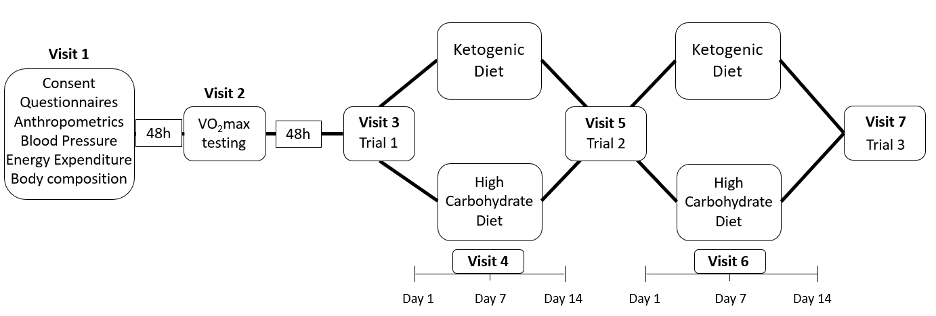
\includegraphics[width=1\linewidth]{figures/figure1} \caption{Figure 1: Study Design. VO~2~max = maximal oxygen consumption}\label{fig:fig1pdf}
\end{figure}

\hypertarget{participants}{%
\subsection{Participants}\label{participants}}

Endurance-trained recreational cyclists and triathletes were recruited
from the local cycling and triathlon community using flyers, social
media, and word of mouth. A total of 46 individuals were assessed for
eligibility, 19 of which were unable to begin the study due to COVID-19
restrictions on in-person research. A further six participants started
the study, but were unable to finish the entire protocol due to these
restrictions. Thus, six participants (m = 2, f = 4) completed the study.
The study was unable to achieve the originally estimated sample size of
30 participants due to data collection restrictions caused by the
COVID-19 pandemic. Figure 2 presents a CONSORT diagram for the present
study

\begin{figure}[H]
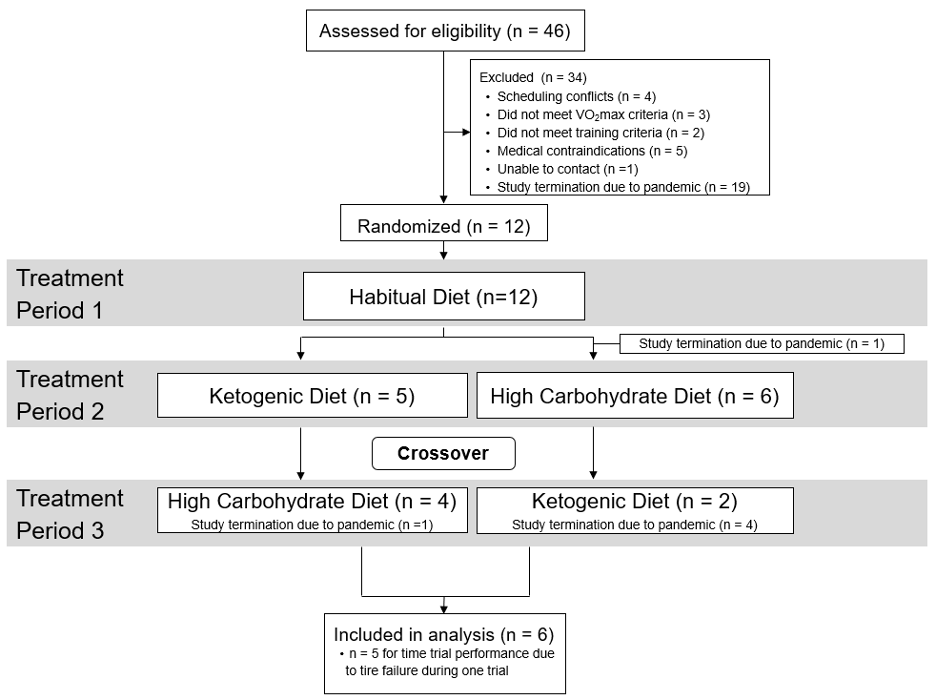
\includegraphics[width=1\linewidth]{figures/figure2} \caption{Figure 2: CONSORT Diagram}\label{fig:fig2pdf}
\end{figure}

Participants were considered endurance trained if they self-reported
\(\geq\) 100 km/wk of cycling for the past year and achieved a
VO\textsubscript{2}max above the 80th percentile for their sex and age
group according to guidelines put forth by the American College of
Sports Medicine (\protect\hyperlink{ref-33}{Sports Medicine, 2018}) with
a 5\% adjustment for comparing cycle ergometry values to the treadmill
derived ACSM norms (\protect\hyperlink{ref-34}{Basset \& Boulay, 2000}).
Participants included one male in Performance Level 2 and one male in
Performance Level 1 as described by Pauw K et al.
(\protect\hyperlink{ref-35}{2013}). Further, our study included three
female participants in Performance Level 3 and one in Performance Level
1 according to criteria established by Decroix et al.
(\protect\hyperlink{ref-36}{2016}). We used relative
VO\textsubscript{2}max as the primary criterion for categorization of
our participants (\protect\hyperlink{ref-36}{Decroix et al., 2016};
\protect\hyperlink{ref-35}{Pauw K et al., 2013}). However, it is
important to note that all participants achieved at least Performance
Level 3 based on weekly mileage and cycling experience. Further, the
male participant classified as Performance Level 2 would have achieved
Performance Level 4 or Performance Level 5 based on absolute or relative
peak power output respectively. Participant characteristics are shown in
Table 1 and have in part been previously reported elsewhere
(\protect\hyperlink{ref-37}{Graybeal et al., 2021}).

\begin{ThreePartTable}
\begin{TableNotes}
\item \textit{Note.} 
\item Mean ± Standard Deviation
\end{TableNotes}
\begin{longtable}[t]{llll}
\caption{\label{tab:tab1pdf}\textbf{Table 1}: Participants Characteristics at Screening.}\\
\toprule
  & Total (n=6) & Male (n=2) & Female (n=4)\\
\midrule
Age (y) & 37.2 ± 12.2 & 41.5 ± 20.5 & 35.0 ± 9.5\\
\addlinespace
Height (cm) & 172.3 ± 10.0 & 183.5 ± 1.0 & 166.8 ± 5.0\\
\addlinespace
Body mass (kg) & 68.5 ± 17.5 & 89.1 ± 7.1 & 58.2 ± 8.3\\
\addlinespace
Body Mass Index (kg/m2) & 22.7 ± 3.4 & 26.5 ± 2.3 & 20.9 ± 2.0\\
\addlinespace
Body fat (\%) & 21.3 ± 4.6 & 21.1 ± 7.2 & 21.4 ± 4.2\\
\addlinespace
Fat-free mass (kg) & 53.8 ± 13.2 & 70.1 ± 0.8 & 45.6 ± 5.0\\
\addlinespace
Fat mass (kg) & 14.7 ± 5.9 & 19.07 ± 7.9 & 12.6 ± 4.2\\
\addlinespace
Max. Oxygen Consumption (mL/kg/min) & 46.8 ± 6.8 & 47.2 ± 6.7 & 46.6 ± 7.9\\
\addlinespace
Max. Oxygen Consumption (L/min) & 3.2 ± 0.9 & 4.2 ± 0.5 & 2.7 ± 0.2\\
\addlinespace
Peak Power Output (W) & 295.5 ± 73.1 & 372.5 ± 74.2 & 257.0 ± 33.7\\
\addlinespace
Peak Power Output (W/kg) & 4.4 ± 0.7 & 4.2 ± 1.2 & 4.5 ± 0.6\\
\addlinespace
Cycling experience (years) & 6.0 ± 4.3 & 6.5 ± 4.9 & 5.8 ± 4.8\\
\addlinespace
Cycling frequency (days/wk) & 4.5 ± 1.0 & 4.5 ± 0.7 & 4.5 ± 1.3\\
\addlinespace
Cycling distance (km/wk) & 225.3 ± 64.2 & 217.0 ± 33.9 & 229.5 ± 80.0\\
\addlinespace
Resting Metabolic Rate (kcals/d) & 1617.3 ± 314.7 & 1999.5 ± 68.6 & 1426.3 ± 132.0\\
\bottomrule
\insertTableNotes
\end{longtable}
\end{ThreePartTable}

Exclusion criteria included the self-reported use of medications or
supplements to lose weight, following a ketogenic (\textless10\% or less
of total energy intake from carbohydrates), a high carbohydrate diet
(\textgreater65\% of total energy intake from carbohydrate), or weight
loss diet. Further, nicotine use or heavy alcohol consumption
(\textgreater14 units of alcohol/week for males; \textgreater7 units of
alcohol/week for females) were considered reasons for exclusion.
Potential participants were also excluded if they self-reported any food
allergies to ingredients used in our test meals. Known cardiovascular
disease was cause for exclusion unless participation was approved by the
participant's cardiologist. Self-reported presence of diabetes, stroke,
anemia, eating disorders, uncontrolled hypertension, or pulmonary,
liver, kidney, and untreated thyroid disease, or orthopedic, arthritis,
or musculoskeletal problems that would have prevented exercise excluded
prospective participants from enrolling in the study. Potential
participants were also excluded if they had undergone surgery that had
lasting effects on swallowing or digestion.

\hypertarget{power-analysis}{%
\subsection{Power Analysis}\label{power-analysis}}

We performed a simulation-based power analysis using the Superpower
package (\protect\hyperlink{ref-38}{Lakens \& Caldwell, 2021}) in R
(\protect\hyperlink{ref-31}{\emph{R Version 4.1.1}, 2021}). Based on
unpublished data collected in our lab in a representative sample, we
expected the time trial to take approximately 60 ± 6 min. The
within-subjects correlation between repeated time trials in our pilot
work was 0.98; high within-subjects correlations (r = 0.89) have been
shown in the existing literature (\protect\hyperlink{ref-18}{Burke et
al., 1985}). To employ a conservative approach, we elected to use the
average of the within-subjects correlation in our pilot work and in
Burke et al. (\protect\hyperlink{ref-18}{1985}), resulting in r = 0.93
for our power analysis. We analyzed finishing times from the past four
years (2015-2018) of the Texas State Time Trial Championships to
establish a practically meaningful effect size. In male and female
athletes of age groups up to 55+ years old, the average finishing time
of the top 10 riders was 61 ± 6 min. On average, an improvement of 1.5
min would have resulted in a rider moving up by one place in the final
standings. Therefore, we decided on a meaningful difference of 90
seconds for our power analysis. All finishing times used in our analysis
can be found at \url{https://osf.io/ujx6e/}. At an alpha level of 0.05,
our power analysis revealed that 30 participants would have yielded 90\%
power for the omnibus linear model for time to completion of the 30-km
time trial. The syntax for the power analysis can be found at
\url{https://osf.io/ujx6e/}. As discussed, we were unable to reach our
desired sample size due to COVID-19 restrictions on in-person research.
Therefore, we do not present any inferential statistics for our primary
outcome measure.

\hypertarget{screening}{%
\subsection{Screening}\label{screening}}

\hypertarget{visit-1}{%
\subsubsection{Visit 1}\label{visit-1}}

Following a 12-hour overnight fast, participants reported the laboratory
for Visit 1, which included completing informed consent and demographic,
behavioral, and health questionnaires. Additionally, participants
underwent anthropometric measurements (height, body mass, waist, and hip
circumference). Further, we assessed participants' body composition
using air displacement plethysmography with measured thoracic lung
volume (BOD POD, COSMED USA Inc., Concord, CA). Following body
composition and anthropometric measurements, we assessed participants'
resting metabolic rate via indirect calorimetry using the ParvoMedics
TrueOne® 2400 metabolic cart (ParvoMedics, Sandy, UT, USA) with a
ventilated hood system.

\hypertarget{visit-2}{%
\subsubsection{Visit 2}\label{visit-2}}

At Visit 2, participants performed an incremental exercise test to task
failure to determine VO\textsubscript{2}max using a CompuTrainer®
ergometer (RacerMate Inc., Seattle, WA). Participants were instructed to
refrain from any exercise in the 24 hours leading up to
VO\textsubscript{2}max testing and to only perform light or moderate
exercise 24-48 hours before testing.

\hypertarget{experimental-trials}{%
\subsection{Experimental Trials}\label{experimental-trials}}

Participants reported to the laboratory following a 12-hour overnight
fast. Additionally, they performed only light to moderate exercise 24-48
hours prior to testing and refrained from all exercise in the 24 hours
leading up to the experimental trials. Upon arrival, participants
underwent measurements of body mass, capillary beta-hydroxybutyrate
concentration, and an ultrasonic assessment of the right and left rectus
femoris. Following resting measures, participants consumed a liquid test
meal approximately 180 min prior to the start of the time trial. They
were allowed ten minutes to consume the test meal in its entirety; time
to consume the meal was standardized between trials based on the time
taken for consumption of the meal during the initial trial. Following
180 minutes of supine rest and postprandial measures described elsewhere
(\protect\hyperlink{ref-37}{Graybeal et al., 2021}), participants
underwent rectus femoris ultrasound assessment and provided capillary
samples for beta-hydroxybutyrate measurement. Then, they completed a
30-km simulated cycling time trial. A diagram showing all measures
performed during each experimental trial is presented in Figure 3.

\begin{figure}[H]
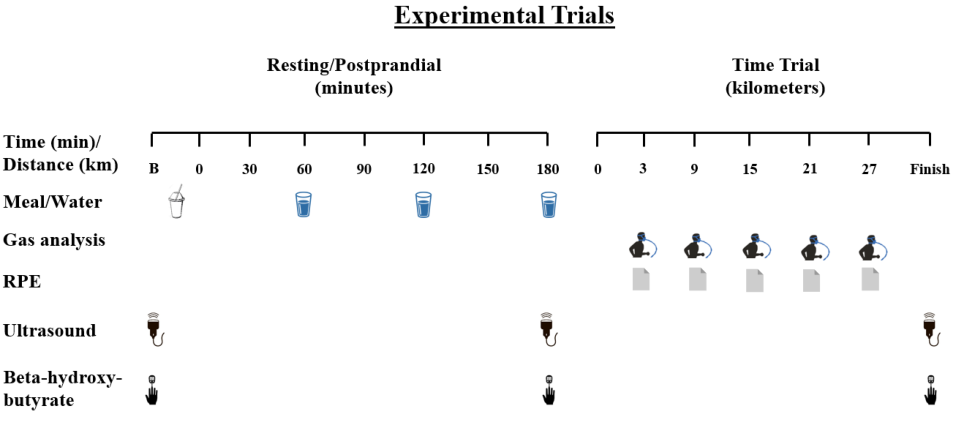
\includegraphics[width=1\linewidth]{figures/figure3} \caption{Figure 3: Experimental Trial Procedures. RPE = Rating of Perceived Exertion}\label{fig:fig3pdf}
\end{figure}

\hypertarget{dietary-interventions-compliance-and-training}{%
\subsection{Dietary Interventions, Compliance, and
Training}\label{dietary-interventions-compliance-and-training}}

Dietary interventions, compliance measures, and experimental controls
regarding physical activity are described in detail elsewhere
(\protect\hyperlink{ref-37}{Graybeal et al., 2021}). We did not
prescribe energy and nutrient intake during the habitual diet; rather,
participants completed 3-day dietary records to quantify their habitual
intake before Experimental Trial 1. The average energy and macronutrient
content of the habitual diet is shown in Table 2. Thereafter, they
followed a ketogenic (\textless10\% carbohydrate, 75-85\% fat, 15\%
protein) and high carbohydrate diet (\textgreater65\% carbohydrate,
\textless20\% fat, 15\% protein) in randomized order. Similar to
previous studies, we did not include a washout period between diets to
maximize participant retention (\protect\hyperlink{ref-39}{Hall et al.,
2021}). Considering that adaptations to the ketogenic diet can be rapid
and quickly reversed by reintroducing carbohydrate, we believe that the
lack of a washout period did not have undue influence on our results
(\protect\hyperlink{ref-40}{Shilpa \& Mohan, 2018}). We considered
participants to be compliant with the diet if they met carbohydrate
macronutrient percentages on at least 80\% of days. Compliance with the
diets was assessed by a registered dietitian via daily diet logging and
daily check-ins using mobile applications (WhatsApp, WhatsApp Inc.,
Mountain View, CA; NutritIO, Bucharest, Romania). Further, participants
provided capillary beta-hydroxybutyrate samples at each experimental
trial and seven days into each diet, as well as daily images of urinary
ketone body test strips (VALI, CA) to test for ketosis, i.e., urinary
beta-hydroxybutyrate concentration \(\ge\) 0.5 mmol/L
(\protect\hyperlink{ref-41}{Misra \& Oliver, 2015}). We instructed
participants to attempt to maintain body mass throughout the study and
considered weight maintenance as a body mass loss or gain of no more
than 5\%.

During experimental trials, participants consumed liquid test meals
containing 60\% of the participants' measured Resting Metabolic Rate
(kcals/day). All meals were dairy-based shakes, which have been
described in detail elsewhere (\protect\hyperlink{ref-37}{Graybeal et
al., 2021}). Test meal compositions corresponded to a typical American
Diet, as outlined by Shan et al. (\protect\hyperlink{ref-32}{2019}), for
the habitual diet (31.4\% fat, 53.4\% carbohydrate, 15.2\% protein) and
to the respective dietary interventions following the high carbohydrate
diet (15.7\% fat, 69.1\% carbohydrate, 15.2\% protein) and the ketogenic
diet (75.1\% fat, 9.5\% carbohydrate, 15.4\% protein); test meal volumes
and caloric content were the same across conditions. Test meals were
consumed in the same amount of time in each condition. Participants
consumed standardized amounts of water during the postprandial period
and were provided with and instructed to ingest the same volume of water
during each time trial. We instructed participants to keep their
training levels stable throughout the study. We monitored training using
self-reported written training logs including distance covered, time
spent, and rating of perceived exertion for the session (RPE; 1-10). We
calculated session RPE by multiplying the indicated RPE by the time
elapsed during the session.

\hypertarget{measures}{%
\subsection{Measures}\label{measures}}

\hypertarget{exercise-equipment}{%
\subsubsection{Exercise Equipment}\label{exercise-equipment}}

To ensure familiarity with the exercise equipment and to avoid learning
effects across trials, participants completed all testing on their
personal bicycles mounted to a CompuTrainer® cycling ergometer
(RacerMate Inc., Seattle, WA), which has previously been shown to be
reliable in time trial tasks similar to the present study
(\protect\hyperlink{ref-42}{Sparks et al., 2016}). The CompuTrainer® was
calibrated according to manufacturer's recommendations, and tire
pressure was standardized for each trial at 100 psi or the maximal tire
pressure recommended by the manufacturer. Participants were asked to
remove devices from their bicycles or deactivate any devices that could
give them feedback on their exercise performance, such as power meters
and cycle computers. The only data displayed to participants during the
time trial were distance and gradient of the road.

\hypertarget{vo2max-testing}{%
\subsubsection{\texorpdfstring{VO\textsubscript{2}max
Testing}{VO2max Testing}}\label{vo2max-testing}}

For the 24 hours leading up to testing, participants were asked to
refrain from all exercise. For the initial incremental maximal exercise
test, participants warmed up for 5 min at a self-selected intensity.
Thereafter, participants began the incremental test at a load of 50-100
watts (W). Exercise intensity was increased by 25 W per minute until
task failure. Oxygen uptake (VO\textsubscript{2}) was continuously
monitored using a TrueOne 2400 metabolic cart (Parvo Medics, Sandy, UT,
USA) and heart rate was collected throughout the test using a Polar H7
HR monitor (Polar Inc., Lake Success, NY). VO\textsubscript{2}max was
defined as the highest 30-second VO\textsubscript{2} value obtained
during the test. To ensure validity of the VO\textsubscript{2}max
measurement, participants performed a validation bout at 110\% of their
peak power output achieved in the initial test following at least 15 min
rest as described by Poole \& Jones
(\protect\hyperlink{ref-poole2017measurement}{2017}). Peak power output
was calculated as described by Hawley \& Noakes
(\protect\hyperlink{ref-hawley1992}{1992}):

\[
PPO=P_{final}+\frac{t}{60} \cdot 25
\]

where Pfinal is the highest work rate achieved and t is the time
completed in the final stage. Following a two-minute warmup at 100 W,
participants performed a steady work rate test that achieved exhaustion
within three to six min. If the greatest VO\textsubscript{2} measured
during this validation test did not exceed the VO\textsubscript{2}max
measured during the incremental test, considering a possible
\textasciitilde3\% measurement error based on the equipment used, the
achievement of a VO\textsubscript{2}2 plateau was accepted. When the
VO\textsubscript{2} achieved during validation exceeded that measured
during the incremental test, a new incremental test was performed on a
separate day.

\hypertarget{performance-assessment}{%
\subsubsection{Performance Assessment}\label{performance-assessment}}

Participants completed a simulated 30-km time trial 180 min following
ingestion of the test meal. With their personal bicycle mounted to the
CompuTrainer® and tire pressures standardized, participants performed a
10-minute warm up followed by calibration of the press-on force of the
load generator per manufacturer's guidelines. Participants then
completed the 30-km time trial on a virtual course in the RacerMate One™
software (RacerMate Inc., Seattle, WA). A copy of the course file can be
found at \url{https://osf.io/ujx6e/}. Participants were instructed to
complete the time trial as quickly as possible and were verbally
encouraged throughout the trial. Participants' heart rate was monitored
continuously using a Polar H7 heart rate sensor and chest strap (Polar
Electro Oy, Kempele, Finland). Respiratory gas measurements and ratings
of perceived exertion (RPE) on a 6-20 Borg Scale were collected at 3 km
and every 6 km thereafter.

\hypertarget{respiratory-gas-analysis}{%
\subsubsection{Respiratory Gas
Analysis}\label{respiratory-gas-analysis}}

Respiratory gas measurements were collected using an open circuit
automated gas analysis system (TrueOne2400, Parvo Medics, Sandy, UT).
Participants breathed through a two-way valve (Hans Rudolph, Shawnee,
KS) attached to a 7450 Series Silicone V2TM Oro-Nasal Mask (Hans
Rudolph) for three min at each collection time point. Substrate
oxidation was calculated using the following equations
(\protect\hyperlink{ref-43}{Péronnet \& Massicotte, 1991}), which assume
a non-protein RER:

\[
Carbohydrate \text{  } oxidation \text{  } (g/min) = 4.585 \cdot VCO_2 - 3.226 \cdot VO_2 
\]

\[
Fat \text{  } oxidation \text{  } (g/min) = 1.695 \cdot VO_2 - 1.701 \cdot VCO_2
\]

\hypertarget{muscle-ultrasound}{%
\subsubsection{Muscle Ultrasound}\label{muscle-ultrasound}}

Session fuel percentile was determined using ultrasonic assessment of
the right and left rectus femoris. Session fuel percentile provides an
estimate of the muscle content of glycogen and other constituents based
on the mean pixel intensity of an ultrasound image. Ultrasonic imaging
was performed with a diagnostic high-resolution GE LOGIQ-e (GE
Healthcare, Milwaukee, WI) using a 9L transducer at 8 Hz. Images from
both rectus femoris muscles were taken in triplicate. Ultrasound images
were uploaded via DICOM to a secure cloud-based web application
(MuscleSound Inc, Denver, CO), which analyzes the echogenicity of the
ultrasound image as an estimate of the content of muscle glycogen and
other constituents. This method has been shown to correlate highly with
glycogen content measured by muscle biopsy
(\protect\hyperlink{ref-29}{Hill \& San Millán, 2014};
\protect\hyperlink{ref-44}{Nieman et al., 2015}). However, some studies
have questioned the validity and utility of this technique
(\protect\hyperlink{ref-45}{Bone et al., 2021};
\protect\hyperlink{ref-46}{Routledge et al., 2019}). In the present
study, we investigated whether the MuscleSound® system was able to
detect assumed changes in muscle glycogen content resulting from dietary
interventions and a 30-km time trial. Following recommendations in
personal communications with the company, we used the session fuel
percentile score, which was implemented after publication of the
MuscleSound® position stand on the application of the system
(\protect\hyperlink{ref-47}{\emph{The MuscleHealth Company. Position
Stand. Science and Application}, 2018}).

\hypertarget{resting-metabolic-rate}{%
\subsubsection{Resting Metabolic Rate}\label{resting-metabolic-rate}}

Resting Metabolic Rate was measured by indirect calorimetry using the
TrueOne® 2400 (ParvoMedics, Sandy, UT, USA) indirect calorimeter with a
ventilated hood system following a 12-hour overnight fast from food,
supplements, and medication and a 24-hour abstinence from exercise. The
first ten min of the 30 min measurement period were used to allow the
participants to achieve resting status; the final 15 min were used for
analysis.

\hypertarget{air-displacement-plethysmography}{%
\subsubsection{Air Displacement
Plethysmography}\label{air-displacement-plethysmography}}

Participants entered the BOD POD (COSMED USA Inc., Concord, CA) wearing
a bathing suit or cycling kit with all hair collected into a swim cap.
Thoracic lung volume were measured during the test using the BOD POD
system.

\hypertarget{data-analysis}{%
\subsection{Data Analysis}\label{data-analysis}}

\hypertarget{time-to-completion-and-average-power-output}{%
\subsubsection{Time to Completion and Average Power
Output}\label{time-to-completion-and-average-power-output}}

As described above, the study was powered based on a time to completion
analysis of finishing times at the Texas State Time Trial Championships.
Thus, we deemed time to completion for the present time trial our
primary outcome measure. However, following the completion of three
participants, we identified an error in our protocol that caused
assigned rider weights in the RacerMate One™ software to be incorrect
for some participants/conditions. The software calculates the speed the
avatar achieves on the virtual course using rider weight, bike weight,
road gradient, and measured power output. Thus, several finishing times
were incorrect. Therefore, we present the average power outputs during
the time trial as our measure of endurance performance below. Further,
we discuss considerations regarding the calculations that produce speed
output from power input in the RacerMate One™ software in the Discussion
section. As detailed above, since we did not achieve the desired
statistical power, we only present means and standard deviations for
these outcome measures; inferential statistics are not presented.

\hypertarget{statistical-analysis}{%
\subsubsection{Statistical Analysis}\label{statistical-analysis}}

All analyses were performed in the R statistical environment
(\protect\hyperlink{ref-31}{\emph{R Version 4.1.1}, 2021}). One
participant with missing data for one-time trial (tire failure at 26 km)
was removed from the analysis of average power output. All analysis
scripts and data used in this manuscript can be found at
\url{https://osf.io/ujx6e/}.

\hypertarget{exploratory-analyses}{%
\subsubsection{Exploratory Analyses}\label{exploratory-analyses}}

Missing data for exploratory analyses (e.g., session fuel percentile)
were imputed using the MICE package in R
(\protect\hyperlink{ref-48}{Buuren S \& K, 2011}) using the PAN method
created by Schafer \& Yucel (\protect\hyperlink{ref-49}{2012}).
Exploratory variables were analyzed using a linear mixed-effects model
with a Holm-Bonferroni post hoc test using the lme4 and emmeans packages
in R (\protect\hyperlink{ref-50}{Bates et al., 2019};
\protect\hyperlink{ref-51}{Lenth et al., 2019}). Fixed effects for these
models include diet (habitual, ketogenic, high carbohydrate) and time
trial time points (3km, 9km, 15km, 21km, 27km). Participant intercept
was treated as a random effect. While prior research would have allowed
the generation of directional hypotheses regarding respiratory exchange
ratio, substrate oxidation, and RPE, we treated these variables as
exploratory, since we did not power the study to these variables. Alpha
level was set at 0.05 for all exploratory analyses.

\hypertarget{control-variables}{%
\subsubsection{Control Variables}\label{control-variables}}

Dietary intake, body mass, physical activity, environmental conditions
during the time trial, and capillary beta-hydroxy-butyrate were treated
as control variables. Potential mean differences in body mass by diet
condition, dietary intake, and capillary beta-hydroxybutyrate were
analyzed using linear mixed-effects models as explained above.
Differences in environmental conditions (humidity and fluid intake),
were analyzed using standard linear models. We did not perform
statistical analysis of lab temperature, since the temperature was 22.0
degrees during all but four trials, where the temperature was 21.0
degrees. Potential mean differences in physical activity (total distance
and sRPE) between diet conditions were assessed using paired t-tests.

\hypertarget{assumption-checks}{%
\subsubsection{Assumption Checks}\label{assumption-checks}}

Visual inspection of residual plots confirmed that normality and
homoscedasticity assumptions were met for all analyses.

\hypertarget{interventional-control}{%
\subsubsection{Interventional Control}\label{interventional-control}}

Means and standard deviations for all control variables are reported in
Table 2 and have been in part reported elsewhere
(\protect\hyperlink{ref-37}{Graybeal et al., 2021}).

\begin{ThreePartTable}
\begin{TableNotes}
\item \textit{Note.} 
\item Mean ± Standard Deviation. RPE = rating of perceived exertion 
\end{TableNotes}
\begin{longtable}[t]{llll}
\caption{\label{tab:tab2pdf}\textbf{Table 2}: Control variables for the three diet conditions (n = 6).}\\
\toprule
  & Habitual & Ketogenic & High Carbohydrate\\
\midrule
Total Energy Intake (kcal) & 2140 ± 555 & 2447 ± 509 & 2418 ± 652\\
\addlinespace
Carbohydrate (\% total energy) & 45.8 ± 6.9 & 8.7 ± 2.9 & 63.3 ± 8.8\\
\addlinespace
Fat (\% total energy) & 38.2 ± 7.8 & 64.1 ± 5.4 & 20.8 ± 7.6\\
\addlinespace
Protein (\% total energy) & 16.5 ± 4.2 & 26.0 ± 2.9 & 14.4 ± 3.2\\
\addlinespace
Body Mass (kg) & 68.7 ± 17.5 & 66.4 ± 16.8 & 68.6 ± 17.3\\
\addlinespace
Average Training session RPE (A.U.) & - & 482 ± 225 & 579 ± 262\\
\addlinespace
Total Training Volume (km) & - & 339 ± 165 & 365 ± 188\\
\addlinespace
Fluid Intake During Time Trial (mL) & 383 ± 74 & 352 ± 146 & 343 ± 100\\
\addlinespace
Fasting beta-hydroxybutyrate (mmol/L) & 0.27 ± 14 & 0.99 ± 61 & 0.10 ± 18\\
\addlinespace
Ambient Temperature (°C) & 21.8 ± 0.4 & 21.7 ± 0.5 & 21.8 ± 0.4\\
\addlinespace
Relative Humidity (\%) & 51.3 ± 6.0 & 36.8 ± 8.4 & 36.5 ± 12.2\\
\bottomrule
\insertTableNotes
\end{longtable}
\end{ThreePartTable}

\hypertarget{dietary-intake-and-beta-hydroxybutyrate}{%
\subsubsection{Dietary Intake and
Beta-Hydroxybutyrate}\label{dietary-intake-and-beta-hydroxybutyrate}}

Detailed dietary intake and beta-hydroxybutyrate results are reported
elsewhere (\protect\hyperlink{ref-37}{Graybeal et al., 2021}). Briefly,
participants consumed similar amounts of total daily energy. Further,
participants had the greatest protein intake during the ketogenic when
compared with the habitual and high carbohydrate diets. As intended,
carbohydrate consumption was greatest in the high carbohydrate condition
and lowest in the ketogenic condition. Fat consumption was highest in
the ketogenic and lowest in the high carbohydrate condition.

Capillary beta-hydroxybutyrate was greater following the ketogenic when
compared with the high carbohydrate and habitual conditions, indicating
successful compliance with the diet. This is further reflected in the
daily urinary ketone measurements during the ketogenic diet, which
averaged 1.82 ± 0.52 mmol/L.

\hypertarget{body-mass}{%
\subsubsection{Body Mass}\label{body-mass}}

Detailed changes in boy mass during the interventions are reported
elsewhere (37). Briefly, participants weighed significantly less
following the ketogenic compared with the habitual and high carbohydrate
diets. There was no significant difference in body mass between the
habitual and the high carbohydrate conditions. It is important to note
that, while all participants lost weight during the ketogenic diet, none
of them surpassed our threshold of 5\% body mass loss.

\hypertarget{training}{%
\subsubsection{Training}\label{training}}

As reported by Graybeal et al. (\protect\hyperlink{ref-37}{2021}),
participants' training was similar between the high carbohydrate and the
ketogenic condition. There were no significant differences in total
kilometers cycled or sRPE when comparing the two diet conditions.

\hypertarget{water-intake-during-the-time-trial}{%
\subsubsection{Water Intake During the Time
Trial}\label{water-intake-during-the-time-trial}}

Water intake during the time trial was similar between conditions,
\(F(2, 15) = 0.214, p = 0.810, \eta^2_p = 0.028\). Participants consumed
383 ± 74 mL, 352 ± 146 mL, and 343 ± 100 mL of water during the
habitual, ketogenic, and high carbohydrate conditions respectively.

\hypertarget{environmental-conditions-during-the-time-trial}{%
\subsubsection{Environmental Conditions During the Time
Trial}\label{environmental-conditions-during-the-time-trial}}

Temperature in the lab was consistent across all trials averaging 21.8 ±
0.4 °C during the habitual, 21.7 ± 0.5 °C during the ketogenic, and 21.8
± 0.4 °C during high carbohydrate conditions. There was a significant
effect of condition on relative humidity during the time trial,
\(F(2, 15) = 5.037, p = 0.021, \eta^2_p = 0.402\). Humidity was greatest
during the habitual condition (51.3 ± 6.0 \%); it was similar between
ketogenic (36.8 ± 8.4 \%) and high carbohydrate conditions (36.5 ± 12.3
\%).

\hypertarget{results}{%
\section{Results}\label{results}}

\hypertarget{cycling-performance}{%
\subsection{Cycling Performance}\label{cycling-performance}}

\hypertarget{average-power-output}{%
\subsubsection{Average Power Output}\label{average-power-output}}

Five participants completed all three time trials (m = 1, f = 4). One
additional participant completed the time trial in the habitual and high
carbohydrate conditions but had to abort the trial in the ketogenic diet
condition due to a tire failure at 26 km; he completed all other
measures in the ketogenic condition. Average power output during the
time trial was greatest following the high carbohydrate diet (199.7 ±
92.2 W), followed by the habitual (188.0 ± 80.6 W) and ketogenic diets
(172.0 ± 93.2 W). A boxplot of average power outputs is presented in
Figure 4.

\hypertarget{physiological-responses-during-the-time-trial}{%
\subsection{Physiological Responses During the Time
Trial}\label{physiological-responses-during-the-time-trial}}

\hypertarget{oxygen-consumption}{%
\subsubsection{Oxygen Consumption}\label{oxygen-consumption}}

VO\textsubscript{2} during the time trial was similar in all conditions
across all time points. During the habitual and high carbohydrate
condition, participants relative VO\textsubscript{2} was 29.9 ± 7.1
ml/kg/min (63.8 ± 10.0\% VO\textsubscript{2}max) and 29.9 ± 7.1
ml/kg/min (63.6 ± 6.9 \% VO\textsubscript{2}max) respectively. In the
ketogenic condition, participants cycled at 58.6 ± 15.4 \% of their
VO\textsubscript{2}max (27.8 ± 7.1 ml/kg/min). There were no main
effects for condition, \(F(2, 69) = 1.853, p = 0.165, \eta^2_p = 0.05\),
or time, \(F(4, 69) = 0.995, p = 0.416, \eta^2_p = 0.05\), and no time x
condition interaction \(F(8, 69) = 0.556, p = 0.810, \eta^2_p = 0.06\).

\begin{figure}[H]
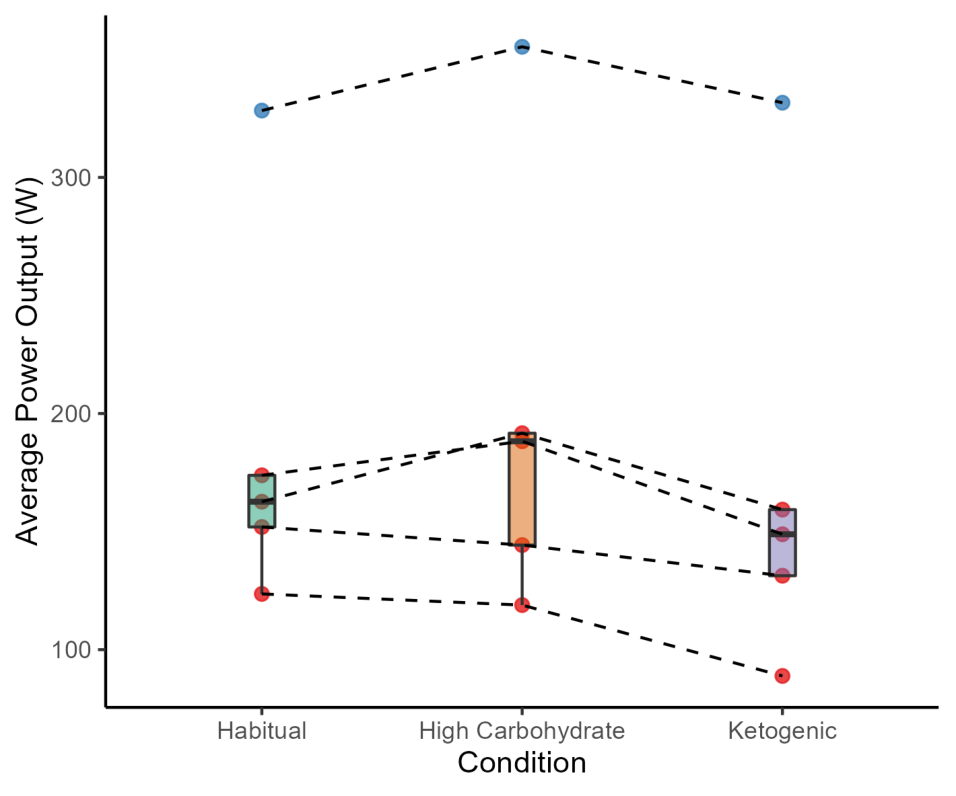
\includegraphics[width=1\linewidth]{figures/figure4} \caption{Figure 4: Average Power Output During the Time Trial (n = 5). Red Circles = Female Participants; Blue Circles = Male Participant.}\label{fig:fig4pdf}
\end{figure}

\hypertarget{heart-rate}{%
\subsubsection{Heart Rate}\label{heart-rate}}

There was no main effect for condition,
\(F(2, 69) = 0.387, p = 0.680, \eta^2_p = 0.01\), and no time by
condition interaction, \(F(8, 69) = 0.270, p = 0.974, \eta^2_p = 0.03\),
for heart rate during the time trial. Participants' heart rate was 163 ±
17 beats/min, 161 ± 22 beats/min, and 162 ± 21 during habitual,
ketogenic, and high carbohydrate conditions respectively. Mean heart
rate rose throughout all trials (3km: 159 ± 17 beats/min; 27km: 167 ± 23
beats/min), but this increase was not statistically significant,
\(F(4, 69) = 2.439, p = 0.055, \eta^2_p = 0.12\).

\hypertarget{substrate-oxidation}{%
\subsubsection{Substrate Oxidation}\label{substrate-oxidation}}

There were main effects for condition
(\(F(2, 69) = 118.178, p < 0.001, \eta^2_p = 0.77\)) and time
(\(F(4, 69) = 6.855, p < 0.001, \eta^2_p = 0.28\)) for carbohydrate
oxidation, but not time x condition interaction
(\(F(8, 69) = 1.177, p = 0.326, \eta^2_p = 0.12\)). During the ketogenic
condition, participants oxidized significantly more carbohydrate
compared with the habitual (Mean Difference {[}MD{]} = -1.11 g/min; 95\%
CI {[}95CI{]} = -1.37, -0.86; t(69) = -10.856; p \textless{} 0.001) and
high carbohydrate conditions (MD = -1.53 g/min; 95CI = -1.78, -1.28;
t(69) = -14.9; p \textless{} 0.001). Additionally, carbohydrate
oxidation was significantly greater in the high carbohydrate condition
compared with habitual condition (MD = 0.42 g/min; 95CI = 0.06, 1.58;
\(t(69) = 3.41; p < 0.001\)). Across all conditions, carbohydrate
oxidation decreased significantly following the 3km measurement (1.87 ±
0.75 g/min) with the lowest average carbohydrate oxidation measured at
21km (1.54 ± 0.76. g/min). Fat oxidation opposed the pattern of
carbohydrate oxidation: it was greatest in ketogenic (0.62 ± 0.11
g/min), followed by the habitual (0.32 ± 0.11 g/min), and the high
carbohydrate conditions (0.14 ± 0.11 g/min),
\(F(2, 69) = 69.101, p < 0.001, \eta^2_p = 0.74\). Averaged across
conditions, fat oxidation was lowest at 3km (0.26 ± .12 g/min) and
highest at 15km (0.41 ± 0.12 g/min); a main effect for time was
observed, \(F(4, 69) = 3.629, p = 0.010, \eta^2_p = 0.17\). There was no
time x condition interaction for fat oxidation,
\(F(8, 69) = 0.445, p = 0.890, \eta^2_p = 0.05\). Individual substrate
oxidation responses during the time trial are presented in Figure 5.

\begin{figure}[H]
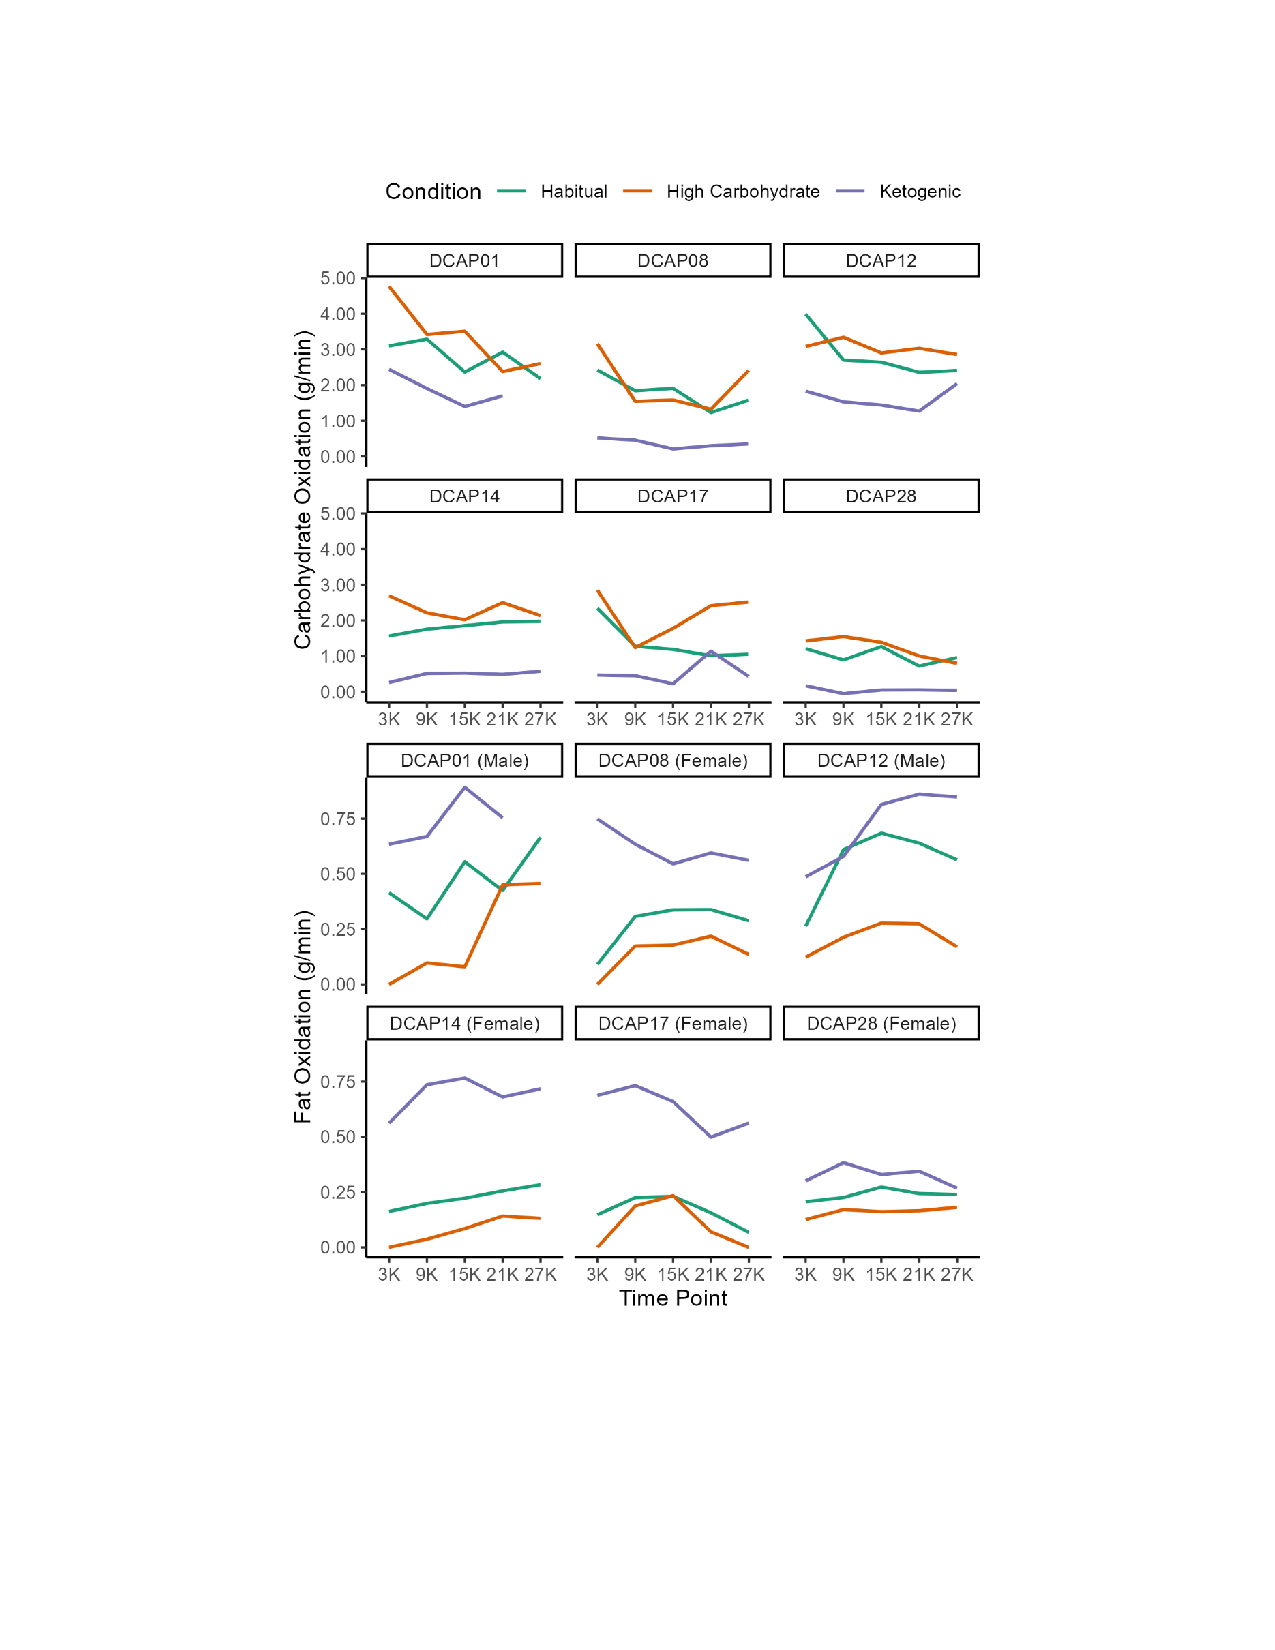
\includegraphics[width=1\linewidth]{figures/figure5} \caption{Figure 5: Individual Substrate Oxidation Responses During the Time Trial.}\label{fig:fig5pdf}
\end{figure}

\hypertarget{perceived-exertion}{%
\subsubsection{Perceived Exertion}\label{perceived-exertion}}

RPE was similar across all three conditions,
\(F(2, 69) = 2.244, p = 0.114, \eta^2_p = 0.06\); participants reported
RPE of 14.5 ± 1.2 for the habitual, 14.9 ± 0.8 for the ketogenic, and
15.0 ± 1.1 for the high carbohydrate condition. Perceived exertion
significantly increased throughout the trial from 13.1 ± 1.2 at 3km to
16.3 ± 1.0 at 27km (time main effect:
\(F(4, 69) = 23.655 p < 0.001, \eta^2_p = 0.58\)). Individual RPE
responses throughout the time trial are shown in Figure 6.

\begin{figure}[H]
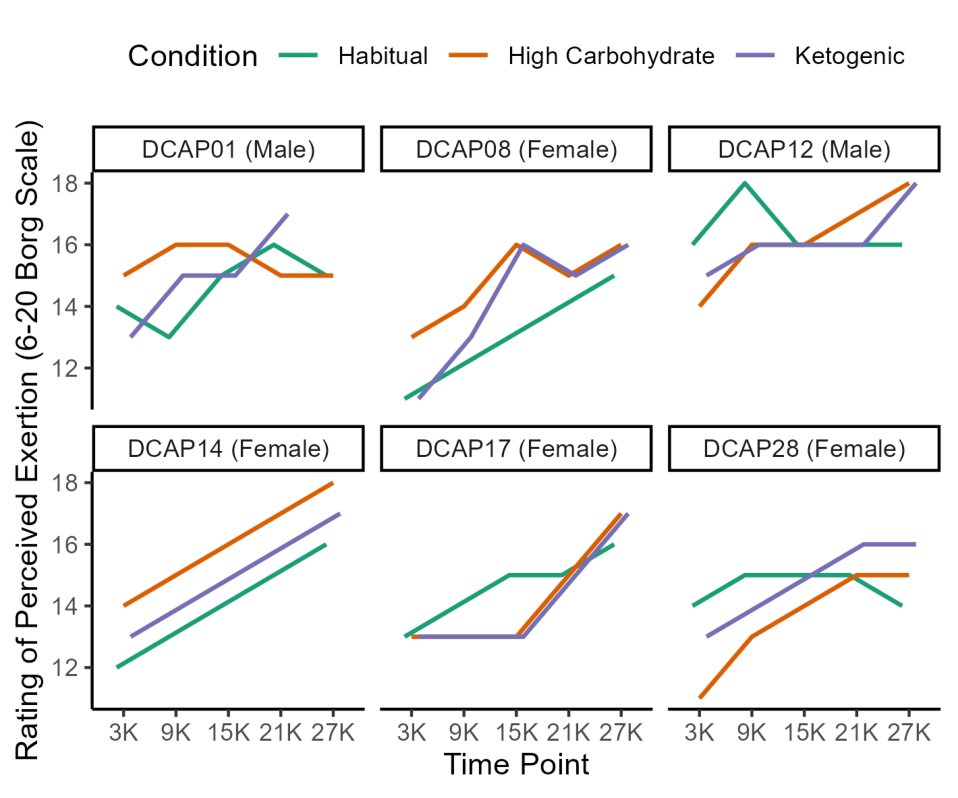
\includegraphics[width=1\linewidth]{figures/figure6} \caption{Figure 6: Individual Rating of Perceived Exertion Responses During the Time Trial.}\label{fig:fig6pdf}
\end{figure}

\hypertarget{muscle-ultrasound-1}{%
\subsubsection{Muscle Ultrasound}\label{muscle-ultrasound-1}}

Figure 7 shows estimated mean differences in session fuel percentile by
condition and time following 100 imputations of missing data using the
MICE package with the PAN method, as described above. Pooled estimates
across the 100 imputations were compatible with a lower session fuel
percentile following two weeks of the ketogenic diet compared with the
habitual diet, MD = -10.0, 95CI {[}-21.0, 0.6{]}, p = 0.063. Similarly,
pooled estimates were compatible with lower session fuel percentile
following the time trial compared with baseline measures, MD = -8.8,
95CI {[}-19.0, 1.3{]}, p = .0085. Session fuel percentile was similar
between habitual and high carbohydrate conditions, as well as between
baseline and pre time trial measures. There appeared to be no
interactions between condition and time.

\begin{figure}[H]
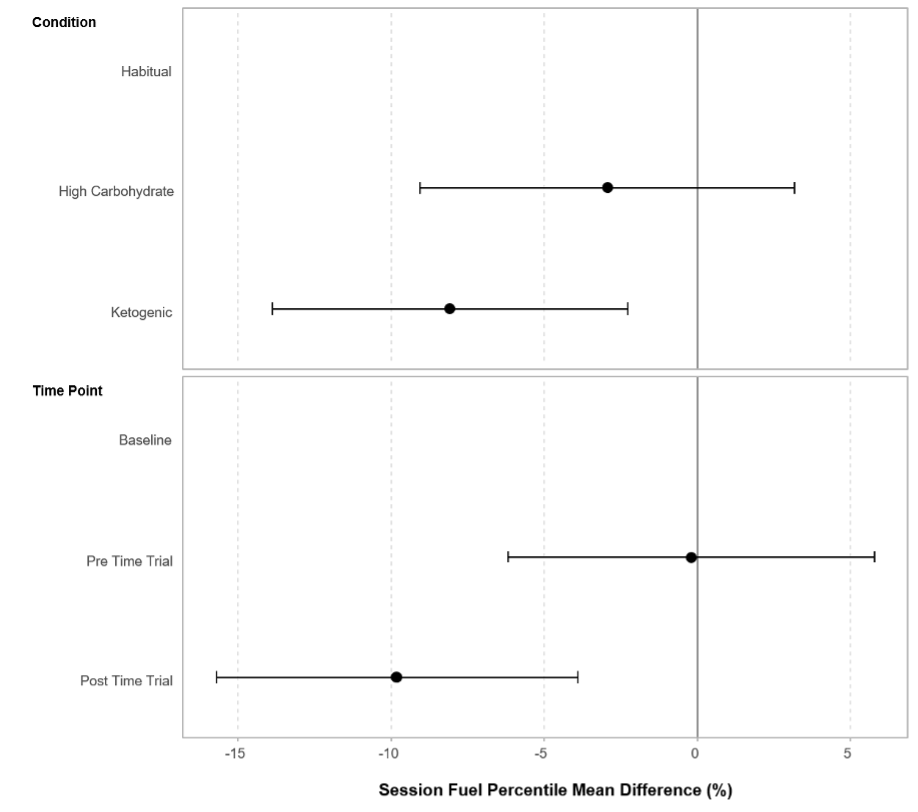
\includegraphics[width=1\linewidth]{figures/figure7} \caption{Figure 7: Estimated Mean Difference in Session Fuel Percentile (n = 6) following 100 imputations of missing data. Error bars represent 95\% Confidence Intervals. Baseline = Fasted; Pre Time-Trial = 180 min following the test meal, immediately prior to the Time Trial; Post Time Trial = immediately following the Time Trial.}\label{fig:fig7pdf}
\end{figure}

\hypertarget{discussion}{%
\section{Discussion}\label{discussion}}

Our results suggest that recreational endurance athletes' power output
during a cycling time trial is potentially reduced following 14 days of
a ketogenic diet when compared with 14-days of a high carbohydrate diet.
This reduction suggests that the observed increase in fat oxidation
during the time trial did not translate to a performance improvement or
maintenance. This could be in part due to reduced muscle glycogen
availability prior to the time trial following the ketogenic diet, which
we observed in the form of decreased session fuel percentile measured
using skeletal muscle ultrasound.

Our findings are in accordance with Burke et al.
(\protect\hyperlink{ref-19}{2017}, \protect\hyperlink{ref-20}{2020}),
who demonstrated endurance performance decrements following a ketogenic
diet despite increased fat oxidation, which they attributed to reduced
exercise economy. While we were unable to directly assess cycling
efficiency due to our protocol, this could be a potential mechanism
explaining the decreased power output during the ketogenic diet
condition in the present study. Studies investigating longer and
lower-intensity exercise tasks have demonstrated potential benefits of
the ketogenic diet on endurance performance
(\protect\hyperlink{ref-7}{Lambert et al., 1994};
\protect\hyperlink{ref-22}{McSwiney et al., 2018}). While lower than
originally expected, participants in the present study worked at higher
relative intensities for shorter durations compared with those
investigations. Thus, it appears that endurance athletes might benefit
or experience no performance decrements following a ketogenic diet when
competing in longer, lower-intensity events, while adverse effects might
arise during shorter, higher-intensity tasks. A recent review by
McSwiney et al. (\protect\hyperlink{ref-52}{2019}) details the effect of
KD on a variety of exercise tasks across different populations.

The increase in fat oxidation rates exhibited by participants in the
present study was lower than what has been reported by other
investigators (\protect\hyperlink{ref-6}{Carey et al., 1985}), while
overall substrate oxidation patterns were similar to the existing
literature (\protect\hyperlink{ref-18}{Burke et al., 1985},
\protect\hyperlink{ref-19}{2017}, \protect\hyperlink{ref-20}{2020},
\protect\hyperlink{ref-16}{2021}; \protect\hyperlink{ref-6}{Carey et
al., 1985}; \protect\hyperlink{ref-21}{Durkalec-Michalski et al., 2019};
\protect\hyperlink{ref-22}{McSwiney et al., 2018};
\protect\hyperlink{ref-23}{Prins et al., 2019};
\protect\hyperlink{ref-24}{Stepto et al., 2002};
\protect\hyperlink{ref-17}{Volek et al., 2016}). However, it is
important to note that we measured substrate oxidation during a
self-paced time trial, rather than during a constant-load exercise task.

While some studies have questioned the validity and utility of using
skeletal muscle ultrasound to estimate muscle glycogen content
(\protect\hyperlink{ref-45}{Bone et al., 2021};
\protect\hyperlink{ref-46}{Routledge et al., 2019}), we successfully
detected expected decreases in muscle ``fuel'' using the MuscleSound®
session fuel percentile score. Although our analyses did not achieve
statistical significance, we observed strong directional results
suggesting reduced muscle fuel following the ketogenic diet as well as
following the time trial across all conditions. While we did not measure
muscle glycogen content directly, and thus cannot speak to the
relationship between session fuel percentile and muscle glycogen
directly, we believe that SFP is a measure that is sensitive enough to
detect changes induced by exercise and diet. Due to its non-invasive
nature and ease of application, this ultrasonic technique appears to be
a valuable tool that allows athletes and practitioners to estimate
muscle ``fuel'' changes in response to dietary and exercise
interventions.

\hypertarget{methodological-insights-and-considerations}{%
\subsection{Methodological Insights and
Considerations}\label{methodological-insights-and-considerations}}

\hypertarget{cycle-ergometer}{%
\subsubsection{Cycle Ergometer}\label{cycle-ergometer}}

Based on participant feedback during previous studies and pilot work as
well as to minimize learning effects, we chose to use the CompuTrainer®
cycle ergometer as our testing device. This allowed participants to
mount their own bicycle to the ergometer maximizing familiarity with the
equipment. In prior work in our laboratory, some participants had voiced
concerns that bicycle fit was suboptimal with other ergometers, such as
the Velotron Pro (RacerMate Inc., Seattle, WA) and Monark Ergomedic 894e
(Monark, Sweden). In a meta-analysis by Hopkins et al.
(\protect\hyperlink{ref-53}{2001}), cycle ergometers that allowed
participants to use their own bicycles produced some of the smallest
coefficients of variation in the study. Participants in the present
study expressed that they favored using their own equipment over using
other ergometers, validating our choice of equipment.

However, certain challenges can come with the use of ergometers that
allow participants to use their own bicycles. First, tire inflation
pressure, and press-on force between the tire and the friction roller of
the load generator must be standardized for each condition between
conditions. The manufacturer's manual for the CompuTrainer® suggests
inflating tires to the maximum rated tire pressure and provides a guide
for setting the POF based on maximal road gradients or maximal expected
power output during the exercise bout. We decided to standardize tire
pressure at 100 psi unless the tires were rated for lower pressure.
However, unbeknownst to the investigators present at the trial, one of
our participants used an inner tube in a tubeless tire during one time
trial, causing over inflation and tire failure. This illuminates another
challenge in allowing participants to use their own bicycles: the need
to ensure that participants don't make changes to their equipment
between trials. One of our participants changed tires between
conditions; the new tires were rated at a lower pressure than the ones
he used in the initial trial. However, the participant had discarded the
old tires, thus making it impossible to keep tire pressure constant
across trials. Data for this participant are not included in this
manuscript, since we had to terminate the study prior to his final
experimental trial due to COVID-19 regulations.

\hypertarget{performance-measure}{%
\subsubsection{Performance Measure}\label{performance-measure}}

To maximize external validity, we decided to use a time trial that was
similar in length (time) to what our participants typically experience
in competition. To align our statistical inference with this strategy,
we powered our study to be able to detect a practical meaningful
difference of 90 seconds between the high carbohydrate and ketogenic
conditions, which, on average, reflected an improvement of one position
in the final standings of the Texas State Time Trial Championships
across the past four years. Thus, we selected time to completion as our
primary outcome measure. While we have used time to completion
successfully in previous work using the Velotron and Monark 894e, the
use of this measure with the CompuTrainer® created additional
challenges. As described above, an error in our protocol caused
inconsistencies in the rider weight used during CompuTrainer® setup.
While the RacerMate One™ software manual provides load curves for the
ergometer, we were unable to determine the exact formula to translate
power output (W) to speed (km/h); one factor influencing this is the
built-in Drag FactorTM function, which allows users to set a percentage
based ``drag factor'' equivalent to an estimated coefficient of
aerodynamic drag multiplied by the frontal area of the rider. The
default value for this and rolling resistance are unknown to the
authors. Our initial strategy was to recalculate finishing times for
each participant by using the speed achieved per watt measured during
the initial time trial (following their habitual diet). We applied this
speed-per-watt factor to the measured power outputs for all other trials
to recalculate finishing times (Supplemental Table S1). Calculation
scripts and speed-per-watt data for each rider by road gradient can be
found at \url{https://osf.io/ujx6e/}.

Using the crude estimation of speed-per-watt employed for our
recalculation of time to completion, it appears that even when setting
the rider weight and press-on-force to nearly identical values a
meaningful difference in speed and finishing time arises. Participant 17
completed the time trial in the ketogenic condition (rider weight: 68.0
kg; bike weight: 10 kg; POF: 3.06 lbs.; drag factor: 100\%) and high
carbohydrate condition (rider weight: 68.0 kg; bike weight: 10 kg;
press-on-force: 3.07; drag factor: 100\%) with nearly identical settings
but received meaningfully different speed-per-watt values. This is in
part due to the increase in coefficient of aerodynamic drag with
increasing speed, as the wind resistance experienced by a rider becomes
greater at higher speed. With the participant riding slower during the
time trial in the ketogenic condition, the software correctly generated
greater speed-per-watt in this condition compared with the high
carbohydrate condition. To control this factor and to further
investigate the speed achieved for the power applied, we analyzed
speed-per-watt at different power outputs across the two trials.
Further, we compared these numbers to a model of overground road cycling
(\protect\hyperlink{ref-54}{Gribble, 2021}), which allows manual entry
of all parameters associated to cycling (Figure 8).

We limited the analysis to flat stretches of the TT to eliminate the
effect of road gradient and only included power outputs between 100 W
and 200 W. It was apparent, that speed-per-watt values fluctuated
greatly immediately following return from a descent to a flat stretch on
the course After removing the 20 seconds following each descent and
large outliers based on visual inspection of the graph, we fit a power
function for all three analyses.

\begin{figure}[H]
\includegraphics[width=1\linewidth]{figures/figure8} \caption{Figure 8: Speed-per-Watt at Different Power Outputs.}\label{fig:fig8pdf}
\end{figure}

\newpage

Even small differences in the speed-per-watts conversion can have
meaningful effects on finishing time during a simulated time trial (see
Supplemental Table S2) At a fictitious power output of 150 in a flat
time trial, the conversion alone would lead to a difference of 44.4
seconds in time to completion. These conversion calculations were highly
sensitive to the inclusion/exclusion of individual datapoints as the
same power input can result in different instantaneous speed output.
Actual differences might not be as large, as individual data points
account for only one second of the speed achieved. However, in the high
carbohydrate trial shown above, power output was measured at 150W on
flat road sections 41 times, with speed-per-watt ranging from 0.179
km/h/W (26.8 km/h) to 0.202 km/h/W (30.3 km/h). It is important to note,
that despite these challenges, the CompuTrainer® very closely mirrors
the time achieved in an overground road cycling time trial.

Despite some limitations regarding the conversion of power output to
speed and the challenges of standardizing between conditions, we believe
the CompuTrainer® is an effective tool for performance analysis. The
familiarity of participants with their own equipment and the positive
feedback regarding bicycle fit and feel may outweigh any challenges
faced with implementing this performance assessment. Based on our
experience in this project, we recommend using mean power output during
a time trial as the performance outcome variable rather than time to
completion. We also suggest extensive piloting of the time trial course
and protocols to ensure all important factors are kept constant between
conditions. Further, we recommend giving participants written
instructions to avoid any changes to their equipment and checking all
aspects of the bicycle setup (including tires) on the day of the trial.

Additionally, we would recommend researchers employing a repeated
measures design use participant's actual body mass on the day of each
trial as rider weight. Since the RacerMate One™ software accurately
models differences in rider weight, potential benefits from decreased
body mass on cycling speed, especially during uphill sections of a
course, should be captured by the performance assessment.

\hypertarget{nutrition-intervention}{%
\subsection{Nutrition Intervention}\label{nutrition-intervention}}

A multi-week nutrition intervention like the one applied in the present
study requires considerable labor and time from the investigators as
well as personal investment from participants. The following section
discusses insights and considerations regarding the nutritional
intervention.

\hypertarget{diet-tracking-and-meal-planning.}{%
\subsubsection{Diet Tracking and Meal
Planning.}\label{diet-tracking-and-meal-planning.}}

Following dietary interventions like the ones employed in the present
study requires careful tracking of nutrition intake and exercise energy
expenditure. The participants in our study provided verbal feedback that
tracking their dietary intake and finding foods to match the
macronutrient requirements for each diet added a sizeable burden to
their daily routines. With this in mind, it is unsurprising that less
than 20\% of recreational cyclists regularly track their nutritional
intake (unpublished data from a survey study conducted in our
laboratory). In fact, in our pre-study screening questionnaire, none of
the participants in the present study reported tracking total energy
intake or macronutrients nor following a specific diet. It stands to
reason that keeping a record of dietary intake and planning meals to
achieve certain nutritional goals might create a steep barrier for
recreational athletes trying to follow high carbohydrate or ketogenic
diets.

Similarly, participants reported struggling to consume the high
percentage of carbohydrate to fulfill the requirements of the high
carbohydrate diet without resorting to sugary drinks and foods. This
could be one reason why our own findings and those of other researchers
(\protect\hyperlink{ref-58}{Worme et al., 1990}) suggest, that
free-living recreational endurance athletes consume less carbohydrate
than what is recommended for optimizing performance
(\protect\hyperlink{ref-1}{Thomas et al., 2016}). The strongest
experimental design regarding diet adherence would include supplying
food for participants throughout the study. This would take the burden
of diet tracking and meal planning off the participants. However, this
is difficult and costly with a free-living cohort such as ours.

\hypertarget{diet-adherence.}{%
\subsubsection{Diet Adherence.}\label{diet-adherence.}}

Our three-day dietary records indicated that participants followed the
intervention diets as prescribed, with the exception of
higher-than-desired protein intake during the ketogenic diet
(Supplemental Table S1). Yet, based on levels of beta-hydroxybutyrate in
urine and blood during the ketogenic diet, participants met our
requirement of being in a ketogenic state. Based on verbal and written
feedback from our participants, even with the daily feedback they
received from the registered dietitian, participants struggled to find
high-fat foods that limited their intake of protein. However, it appears
that the protein intake in our ketogenic diet condition (26.0 ± 2.9\% of
total energy intake) was similar to what other studies have reported
when participants were allowed to consume protein ad libitum
(\protect\hyperlink{ref-55}{Brehm et al., 2003},
\protect\hyperlink{ref-56}{2005}; \protect\hyperlink{ref-57}{Yancy et
al., 2004}). Thus, allowing ad libitum intake of protein during the
ketogenic diet condition appears to be a practical way to reduce the
burden on participants to find low-protein high-fat foods. To control
for the effect of changes in fat-free body mass, which could have an
impact on exercise performance, we suggest measuring body composition
following each diet, if resources allow it. In the present study,
equipment availability prohibited us from performing these measurements.

\hypertarget{blinding}{%
\subsubsection{Blinding}\label{blinding}}

Blinding of participants to the study condition is impossible in a study
design like the present. Participants' effort during training and
performance assessment could be influenced by preconceived opinions
about the interventions employed. Recent research has shown that
recreational endurance athletes are more aware of the effects of
carbohydrate intake before, during, and after events than the general
public (\protect\hyperlink{ref-59}{Sampson et al., 2021}). Thus,
participants might have expected to perform worse during the ketogenic
diet condition. This became apparent in the present study from verbal
comments by the participants, who mentioned not looking forward to
completing the ketogenic diet condition. Additionally, during the
ketogenic diet, they reported feeling like they could not produce the
same amount of power and fatiguing more quickly during training rides.
One participant completed the time trial approximately 13 min slower
during the ketogenic condition than during the habitual and high
carbohydrate conditions. This participant specifically expressed feeling
fatigued during the ketogenic diet. It is unclear whether a preconceived
notion of the ketogenic diet on endurance performance might have
impacted the participant's effort during the time trial or whether the
participant truly experienced such strong effects of the diet.

\hypertarget{statistical-analysis-1}{%
\subsection{Statistical Analysis}\label{statistical-analysis-1}}

\hypertarget{sample-heterogeneity-and-statistical-power}{%
\subsection{Sample Heterogeneity and Statistical
Power}\label{sample-heterogeneity-and-statistical-power}}

Our goal for the present study was to collect data from men and women
across a wider age-range than previously reported in the literature.
However, this has important implications on statistical power. Based on
our analysis of the Texas State Time Trial Championships, finishing
times and standard deviations of the top 10 athletes in male and female
age groups up to 55+ years old (61 ± 6 min) was similar to pilot work on
the CompuTrainer® course in our own lab (60 ± 6). However, our final
sample comprised athletes with much greater heterogeneity in the main
performance outcome. This sample heterogeneity has a drastic impact on
statistical power in a frequentist framework {[}Heidel
(\protect\hyperlink{ref-60}{2016});61{]}.

We attempted to limit sample heterogeneity by requiring minimum training
experience and distance along with a VO\textsubscript{2}max criterion
for enrollment in the study. Average time to completion of the time
trial was similar to what we expected, but standard deviations in our
sample ranged from 8.0 min (habitual condition) to 13.2 min (ketogenic
condition). Simply raising the standard deviation in our power analysis
from 6.0 to 10.2 (average of our observed standard deviations), while
leaving all other parameters the same would decrease statistical power
for the omnibus test with 30 participants from 90\% to 45\%. One avenue
to further limit this heterogeneity and increase statistical power,
would be employing a time trial as part of the screening process to
ensure participants can complete the course in a predetermined maximal
time or at a predetermined minimal average power output. This trial
could also serve as a familiarization trial for participants to become
accustomed to the laboratory and the bike setup.

\hypertarget{analysis-options.}{%
\subsubsection{Analysis Options.}\label{analysis-options.}}

A common strategy to analyze data like the present is to employ repeated
measures analysis of variance (RM-ANOVA). However, other fields
including psychology, biology, and medicine, have transitioned to using
linear mixed-effects models for designs similar to ours
(\protect\hyperlink{ref-62}{Boisgontier \& Cheval, 2016}). In the
following section we present different analysis options for our primary
outcome (time to completion) and for one example of a secondary outcomes
(carbohydrate oxidation). To avoid reporting inferential statistics
based on observed data of our primary outcome, we used simulated data to
show the different analysis options. All simulations and analysis
scripts can be found here: \url{https://osf.io/ujx6e/}

We investigated the outcome of three statistical methods to analyze our
primary outcome (TTC) with simulated data based on the following
parameters using the faux package in R
(\protect\hyperlink{ref-63}{DeBruine et al., 2021}):

\begin{itemize}
\tightlist
\item
  n = 18
\item
  Habitual condition: \(\mu\) = 61.0 min; \(\sigma\) = 8.0 min
\item
  High carbohydrate condition: \(\mu\) = 60.0 min; \(\sigma\) = 9.0 min
\item
  Ketogenic condition: \(\mu\) = 62.5 min; \(\sigma\) = 10.5 min
\end{itemize}

These parameters are loosely based on our actual data in combination
with the practically meaningful effect size of 90 seconds discussed
above. The three methods investigated were: 1) linear mixed-effects
models using the lme4 package, 2) standard RM-ANOVA using the afex
package, and 3) analysis of covariance (ANCOVA), as recommended by Senn
(\protect\hyperlink{ref-64}{2006}) using the rstatix package
(\protect\hyperlink{ref-65}{rstatix, 2021}). As an example of the
secondary outcome analysis, we chose observed data for carbohydrate
oxidation and analyzed them using 1) linear mixed-effects models and 2)
condition x time RM-ANOVA. Inferential statistics for all analyses are
shown in Supplemental Table S3.

To further analyze statistical outcomes of these strategies, we
investigated pairwise comparisons of the estimated marginal mean
differences using the emmeans and statix packages. Results for time to
completion are shown in Supplemental Table S4. We used a Holm correction
for multiple comparisons and a Bonferroni correction for the 95\%
confidence intervals reported.

All three strategies result in similar omnibus test for time to
completion leading to the same inferential interpretation. As expected,
the results for time to completion were nearly identical between models.
Interestingly, there were important differences in the comparisons for
estimated marginal mean differences. While the point estimates for mean
differences between conditions were exactly the same for linear
mixed-effects models and RM-ANOVA, the 95\% CI differed considerably,
leading to a different inferential interpretation (see Supplemental
Table S4) The RM-ANOVA yielded a statistically significant difference
between habitual and high carbohydrate conditions, whereas the linear
mixed-effects model did not. Confidence intervals were wider in the
linear mixed-effects model for the habitual vs.~high carbohydrate
comparison only, but narrower for the other comparisons. One downside to
the ANCOVA approach is that it only allowed for pairwise comparison
between high carbohydrate and ketogenic conditions, since time to
completion from the time trial in the habitual condition was used as a
covariate.

When analyzing carbohydrate oxidation, the omnibus tests for both models
indicated main effects for condition and time without an interaction.
However, only the linear mixed-effects model showed significant
differences in the follow-up pairwise comparisons. The results for post
hoc comparison of estimated marginal means in the linear mixed-effects
model indicated significant difference when comparing carbohydrate
oxidation at the 3km mark in the time trial compared with all other time
points. Interestingly, while the omnibus test for the RM-ANOVA did
indicate a main effect for time, none of the follow-up pairwise
comparisons were statistically significant.

Based on this analysis, we suggest researchers explore the option of
using a linear mixed-effects model in similar designs. The linear
mixed-effects model as applied here allows for a random intercept for
each participant; further benefits of linear mixed-effects model allow
the specification of additional random effects (e.g., participant-level
slopes) and using multiple imputation to handle missing data
(\protect\hyperlink{ref-66}{Harrison et al., 2018}) as employed in our
analysis of the muscle ultrasound data. When deciding between an
RM-ANOVA and an ANCOVA, researchers should consider the study design and
research questions. In the present study, we chose the linear
mixed-effects model over ANCOVA to allow for the pairwise comparison of
all three conditions. It could be argued, that an ANCOVA approach would
have been prudent, since we did not control diet in the habitual
condition; thus, the habitual condition would have lent itself as a true
baseline test used as a covariate in the comparison of high carbohydrate
and ketogenic conditions. However, we believe that this also allowed a
true comparison of a truly habitual condition compared to two controlled
conditions.

\hypertarget{conclusions}{%
\subsection{Conclusions}\label{conclusions}}

We found that participants completed a simulated 30-km time trial at the
lowest mean power output following two weeks of the ketogenic diet. We
also showed that fat oxidation was greatest during the time trial
following the ketogenic diet and lowest following the high carbohydrate
diet. Further, MuscleSound® session fuel percentile, an estimate of
muscle ``fuel'' was lower following the ketogenic diet compared to the
habitual diet; additionally, session fuel percentile was lower following
the time trial compared to fasted baseline measures and 3-hour post-meal
measures. In summary, while this study did not achieve the desired
sample size to make inferential claims about the effects of the
ketogenic and high carbohydrate diets on endurance exercise performance,
we believe that the insights gained from our work could be valuable to
other researchers, athletes, and practitioners. We argue that allowing
participants to use their own bicycles for studies like this on a cycle
ergometer such as the CompuTrainer® reduces learning effects and
minimizes the need for familiarization; further, it provides a valid
measurement of endurance exercise performance, as long as
standardization protocols are followed and appropriate outcome measures
(e.g., mean power output during a time trial) are selected. Further, we
contend that employing linear mixed-effects models should be the
preferred analysis technique for repeated measures design in a
frequentist framework. Linear mixed-effects models offer the option to
include random intercepts at the participant level, which allows
modeling of inter-individual response differences better than using a
fixed intercept. Further, linear mixed-effects models allow multiple
imputation of missing data, providing a route for researchers to use
partial data for participants rather than being forced to delete data
listwise, as is typically done using RM-ANOVA. Depending on the study
design and research question, ANCOVA with baseline performance as the
covariate also offers a valid analysis strategy. In light of the
findings by Burke et al. (\protect\hyperlink{ref-19}{2017},
\protect\hyperlink{ref-20}{2020}) that exercise economy might be reduced
following a ketogenic diet, we suggest that future studies should
include steady-state exercise that allows the measurement of mechanical
efficiency or exercise economy. Finally, we believe that using muscle
ultrasound for a determination of muscle ``fuel'' using the MuscleSound®
session fuel percentile offers a valuable and easy-to-use tool for
practitioners and athletes.

\hypertarget{practical-applications}{%
\subsection{Practical Applications}\label{practical-applications}}

From a practical perspective, following strict diets in the long-term
adds considerable burdens to recreational athletes' lives. Thus, a more
reasonable approach might be to ``fuel for the work required'', as
proposed by Impey et al. (\protect\hyperlink{ref-67}{2018}). In this
paradigm, athletes base their carbohydrate requirements on the work
anticipated and/or performed on a given day. Often, recreational
cyclists will complete longer training sessions (five to six hours) on
weekends and more intense sessions on one or two days during the week.
To minimize the added labor and stress of daily macronutrient and energy
tracking, athletes could increase carbohydrate intake on the day prior
to and during longer and/or more intense training sessions, while eating
entirely ad libitum on days with easier rides. Recreational athletes
using power meters, could calculate energy expenditure based on the
average power produced during a ride. In fact, most exercise tracking
applications, which are popular among this population, already provide
energy expenditure measures based on actual work performed when power
meter data are included. Those who do not use power meters, could use
heart rate and/or the talk test to estimate energy expenditure and
exercise intensity (\protect\hyperlink{ref-68}{Hiilloskorpi et al.,
2003}; \protect\hyperlink{ref-69}{Quinn \& Coons, 2011}). These
calculations would allow recreational athletes to fuel longer and harder
sessions adequately, while not needing to invest the time and energy to
plan and track dietary intake on shorter and easier days.

Single-session carbohydrate restriction for certain low to moderate
intensity workouts, i.e., ``training low'', has been shown to be
effective in augmenting gene expression, cell signaling, and oxidative
enzyme activity related with improved endurance performance
(\protect\hyperlink{ref-70}{Impey et al., 2016},
\protect\hyperlink{ref-67}{2018}). These strategies might be more
feasible and sensible for elite athletes, who typically work with
nutrition professionals and often have already optimized all other
aspects of their training and racing. However, recreational cyclists
looking to use this strategy could implement a higher intensity training
session in the morning followed by carbohydrate restriction and a lower
intensity training session in the evening
(\protect\hyperlink{ref-70}{Impey et al., 2016}).

In summary, recreational athletes looking to improve their cycling
performance using nutrition interventions might be better served by
focusing on ``fueling for the work required''
(\protect\hyperlink{ref-67}{Impey et al., 2018}) and interspersing
occasional training session with low carbohydrate availability than by
trying to implement a daily diet designed to restrict or enhance the
intake of carbohydrate.

\hypertarget{additional-information}{%
\section{Additional Information}\label{additional-information}}

\hypertarget{data-accessibility}{%
\subsection{Data Accessibility}\label{data-accessibility}}

All data and analysis code used for this manuscript are available at
\url{https://osf.io/ujx6e/}

\hypertarget{author-contributions}{%
\subsection{Author Contributions}\label{author-contributions}}

\begin{itemize}
\tightlist
\item
  Contributed to conception and design: AK, AJG, PPR, JLW, MS
\item
  Contributed to acquisition of data: AK, AJG, PPR, KM, GRA
\item
  Contributed to analysis and interpretation of data: AK, AJG, MS
\item
  Drafted and/or revised the article: AK, AJG, PPR, KM, GRA, JLW, RB-T,
  MS
\item
  Approved the submitted version for publication: AK, AJG, PPR, KM, GRA,
  JLW, RB-T, MS
\end{itemize}

\hypertarget{conflict-of-interest}{%
\subsection{Conflict of Interest}\label{conflict-of-interest}}

Authors have no conflicts of interest to declare.

\hypertarget{funding}{%
\subsection{Funding}\label{funding}}

This work was supported in part by the Harris College of Nursing \&
Health Sciences Graduate Student Research Grant.

\hypertarget{acknowledgments}{%
\subsection{Acknowledgments}\label{acknowledgments}}

We would like to acknowledge Sadie Oakley, Emma Kate Wichman, Jordy
Trudel, Megan Conger, Rachel Huther, and Mackenzie Minnick for their
contribution to data collection. Further, we would like to thank all
participants for their time and efforts.

\hypertarget{preprint}{%
\subsection{Preprint}\label{preprint}}

The pre-publication version of this manuscript can be found on
SportRxiv: \url{https://doi.org/10.51224/SRXIV.19}

\newpage

\hypertarget{references}{%
\section{References}\label{references}}

\parindent0pt 
\setlength{\parskip}{1em}

\hypertarget{refs}{}
\begin{CSLReferences}{1}{0}
\leavevmode\vadjust pre{\hypertarget{ref-34}{}}%
Basset, F. A., \& Boulay, M. R. (2000). Specificity of Treadmill and
Cycle Ergometer Tests in Triathletes, Runners and Cyclists.
\emph{European Journal of Applied Physiology}, \emph{81}, 214--221.
\url{https://doi.org/10.1007/s004210050033}

\leavevmode\vadjust pre{\hypertarget{ref-50}{}}%
Bates, D., Maechler, M., Bolker, B., Walker, S., Singmann, H., Dai, B.,
Scheipl, F., Grothendieck, G., Green, P., Fox, J., Green, P., \& Fox, J.
(2019). \url{https://CRAN.R-project.org/package=lme4}

\leavevmode\vadjust pre{\hypertarget{ref-27}{}}%
Bergström, J., \& Hultman, E. (1967). A Study of the Glycogen Metabolism
During Exercise in Man. \emph{Scandinavian Journal of Clinical and
Laboratory Investigation}, \emph{19}, 218--228.
\url{https://doi.org/10.3109/00365516709090629}

\leavevmode\vadjust pre{\hypertarget{ref-62}{}}%
Boisgontier, M. P., \& Cheval, B. (2016). The ANOVA to Mixed Model
Transition. \emph{Neuroscience \& Biobehavioral Reviews}, \emph{68},
1004--1005. \url{https://doi.org/f83jzs}

\leavevmode\vadjust pre{\hypertarget{ref-45}{}}%
Bone, J. L., Ross, M. L., Tomcik, K. A., Jeacocke, N. A., McKay, A. K.
A., \& Burke, L. M. (2021). The Validity of Ultrasound Technology in
Providing an Indirect Estimate of Muscle Glycogen Concentrations Is
Equivocal. \emph{Nutrients}, \emph{13}, 2371.
\url{https://doi.org/gmmtcg}

\leavevmode\vadjust pre{\hypertarget{ref-55}{}}%
Brehm, B. J., Seeley, R. J., Daniels, D. 'Alessio., SR, \& D.A. (2003).
A Randomized Trial Comparing a Very Low Carbohydrate Diet and a
Calorie-Restricted Low Fat Diet on Body Weight and Cardiovascular Risk
Factors in Healthy Women. \emph{Journal of Clinical Endocrinology and
Metabolism}, \emph{88}, 1617--1623.
\url{https://doi.org/10.1210/jc.2002-021480}

\leavevmode\vadjust pre{\hypertarget{ref-56}{}}%
Brehm, B. J., Spang, S. E., Lattin, B. L., Seeley, R. J., Daniels, D.
'Alessio., SR, \& D.A. (2005). The Role of Energy Expenditure in the
Differential Weight Loss in Obese Women on Low-Fat and Low-Carbohydrate
Diets. \emph{Journal of Clinical Endocrinology and Metabolism},
\emph{90}, 1475--1482. \url{https://doi.org/10.1210/jc.2004-1540.}

\leavevmode\vadjust pre{\hypertarget{ref-4}{}}%
Burke, L. M. (2017). Low Carb High Fat (LCHF) Diets for Athletes --
Third Time Lucky? \emph{Journal of Science and Medicine in Sport},
\emph{20 Suppl 1: S1}. \url{https://doi.org/ghp7b8}

\leavevmode\vadjust pre{\hypertarget{ref-18}{}}%
Burke, L. M., Angus, D. J., Cox, G. R., Cummings, N. K., Febbraio, M.
A., Gawthorn, K., Hawley, J. A., Minehan, M., Martin, D. T., \&
Hargreaves, M. (1985). Effect of Fat Adaptation and Carbohydrate
Restoration on Metabolism and Performance During Prolonged Cycling.
\emph{Journal of Applied Physiology}, \emph{89}, 2413--2421.
\url{https://doi.org/10.1152/jappl.2000.89.6.2413.}

\leavevmode\vadjust pre{\hypertarget{ref-10}{}}%
Burke, L. M., Castell, L. M., Casa, D. J., Close, G. L., Costa, R. J.
S., Desbrow, B., Halson, S. L., Lis, D. M., Melin, A. K., Peeling, P.,
Saunders, P. U., Slater, G. J., Sygo, J., Witard, O. C., Bermon, S., \&
Stellingwerff, T. (2019). International Association of Athletics
Federations Consensus Statement 2019: Nutrition for Athletics.
\emph{International Journal of Sport Nutrition and Exercise Metabolism},
\emph{29}, 73--84. \url{https://doi.org/gjbrp2}

\leavevmode\vadjust pre{\hypertarget{ref-15}{}}%
Burke, L. M., \& Hawley, J. A. (2002). Effects of Short-Term Fat
Adaptation on Metabolism and Performance of Prolonged Exercise.
\emph{Medicine \& Science in Sports \& Exercise}, \emph{34}, 1492--1498.
\url{https://doi.org/10.1097/00005768-200209000-00015}

\leavevmode\vadjust pre{\hypertarget{ref-19}{}}%
Burke, L. M., Ross, M. L., Garvican‐Lewis, L. A., Welvaert, M., Heikura,
I. A., Forbes, S. G., Mirtschin, J. G., Cato, L. E., Strobel, N.,
Sharma, A. P., \& Hawley, J. A. (2017). Low Carbohydrate, High Fat Diet
Impairs Exercise Economy and Negates the Performance Benefit From
Intensified Training in Elite Race Walkers. \emph{Journal of
Physiology}, \emph{595}, 2785--2807.
\url{https://doi.org/10.1113/JP273230.}

\leavevmode\vadjust pre{\hypertarget{ref-20}{}}%
Burke, L. M., Sharma, A. P., Heikura, I. A., Forbes, S. F., Holloway,
M., McKay, A. K. A., Bone, J. L., Leckey, J. J., Welvaert, M., \& Ross,
M. L. (2020). Crisis of Confidence Averted: Impairment of Exercise
Economy and Performance in Elite Race Walkers by Ketogenic Low
Carbohydrate, High Fat (LCHF) Diet Is Reproducible. \emph{PLoS One},
\emph{15}, 0234027. \url{https://doi.org/gg23h5}

\leavevmode\vadjust pre{\hypertarget{ref-16}{}}%
Burke, L. M., Whitfield, J., Heikura, I. A., Ross, M. L. R., Tee, N.,
Forbes, S. F., Hall, R., McKay, A. K. A., Wallett, A. M., \& Sharma, A.
P. (2021). Adaptation to a Low Carbohydrate High Fat Diet Is Rapid but
Impairs Endurance Exercise Metabolism and Performance Despite Enhanced
Glycogen Availability. \emph{Journal of Physiology}, \emph{599},
771--790. \url{https://doi.org/ghvh2b}

\leavevmode\vadjust pre{\hypertarget{ref-48}{}}%
Buuren S, \& K, G.-O. (2011). MICE: Multivariate Imputation by Chained
Equations in R. \emph{Journal of Statistical Software}, \emph{45},
1--67. \url{https://doi.org/10.18637/jss.v045.i03}

\leavevmode\vadjust pre{\hypertarget{ref-6}{}}%
Carey, A. L., Staudacher, H. M., Cummings, N. K., Stepto, N. K.,
Nikolopoulos, V., Burke, L. M., \& Hawley, J. A. (1985). Effects of Fat
Adaptation and Carbohydrate Restoration on Prolonged Endurance Exercise.
\emph{Journal of Applied Physiology}, \emph{91}, 115--122.
\url{https://doi.org/10.1152/jappl.2001.91.1.115}

\leavevmode\vadjust pre{\hypertarget{ref-63}{}}%
DeBruine, L., Krystalli, A., \& faux, H. A. (2021). \emph{Simulation for
Factorial Designs} {[}{[}Online{]}.{]}.
\url{https://CRAN.R-project.org/package=faux}

\leavevmode\vadjust pre{\hypertarget{ref-36}{}}%
Decroix, L., Pauw, K., Foster, C., \& Meeusen, R. (2016). Guidelines to
Classify Female Subject Groups in Sport-Science Research.
\emph{International Journal of Sports Physiology and Performance},
\emph{11}, 204--213. \url{https://doi.org/ggcfjx}

\leavevmode\vadjust pre{\hypertarget{ref-21}{}}%
Durkalec-Michalski, K., Nowaczyk, P. M., \& Siedzik, K. (2019). Effect
of a Four-Week Ketogenic Diet on Exercise Metabolism in Crossfit-Trained
Athletes. \emph{Journal of the International Society of Sports
Nutrition}, \emph{16}, 16.
\url{https://doi.org/10.1186/s12970-019-0284-9}

\leavevmode\vadjust pre{\hypertarget{ref-5}{}}%
Feinman, R. D., Pogozelski, W. K., Astrup, A., Bernstein, R. K., Fine,
E. J., Westman, E. C., Accurso, A., Frassetto, L., Gower, B. A.,
McFarlane, S. I., Nielsen, J. V., Krarup, T., Saslow, L., Roth, K. S.,
Vernon, M. C., Volek, J. S., Wilshire, G. B., Dahlqvist, A., Sundberg,
R., \ldots{} Worm, N. (2015). Dietary Carbohydrate Restriction As the
First Approach in Diabetes Management: Critical review and evidence
base. \emph{Nutrition}, \emph{31}, 1--13.
\url{https://doi.org/10.1016/j.nut.2014.06.011}

\leavevmode\vadjust pre{\hypertarget{ref-12}{}}%
Galbo, H., Holst, J. J., \& Christensen, N. J. (1979). The Effect of
Different Diets and of Insulin on the Hormonal Response to Prolonged
Exercise. \emph{Acta Physiologica}, \emph{107}, 19--32,.
\url{https://doi.org/10.1111/j.1748-1716.1979.tb06438.x.}

\leavevmode\vadjust pre{\hypertarget{ref-14}{}}%
Goedecke, J. H., Christie, C., Wilson, G., Dennis, S. C., Noakes, T. D.,
Hopkins, W. G., \& Lambert, E. V. (1999). Metabolic Adaptations to a
High-Fat Diet in Endurance Cyclists. \emph{Metabolism: Clinical and
Experimental}, \emph{48}, 1509--1517.
\url{https://doi.org/10.1016/s0026-0495(99)90238-x}

\leavevmode\vadjust pre{\hypertarget{ref-37}{}}%
Graybeal, A. J., Kreutzer, A., Rack, P., Moss, K., Augsburger, G.,
Willis, J. L., Braun-Trocchio, R., \& Shah, M. (2021). Perceptions of
Appetite Do Not Match Hormonal Measures of Appetite in Trained
Competitive Cyclists and Triathletes Following a Ketogenic Diet Compared
to a High-Carbohydrate or Habitual Diet: A Randomized Crossover Trial.
\emph{Nutrition Research}, \emph{93}, 111--123.
\url{https://doi.org/gmmtch}

\leavevmode\vadjust pre{\hypertarget{ref-54}{}}%
Gribble, S. (2021). \emph{An Interactive Model-Based Calculator of
Cycling Power vs}.
\url{https://www.gribble.org/cycling/power_v_speed.html}

\leavevmode\vadjust pre{\hypertarget{ref-39}{}}%
Hall, K. D., Guo, J., Courville, A. B., Boring, J., Brychta, R., Chen,
K. Y., Darcey, V., Forde, C. G., Gharib, A. M., Gallagher, I., Howard,
R., Joseph, P. V., Milley, L., Ouwerkerk, R., Raisinger, K., Rozga, I.,
Schick, A., Stagliano, M., Torres, S., \ldots{} Chung, S. T. (2021).
Effect of a plant-based, low-fat diet versus an animal-based, ketogenic
diet on ad libitum energy intake. \emph{Nature Medicine}, \emph{27},
344--353. \url{https://doi.org/10.1038/s41591-020-01209-1.}

\leavevmode\vadjust pre{\hypertarget{ref-66}{}}%
Harrison, X. A., Donaldson, L., Correa-Cano, M. E., Evans, J., Fisher,
D. N., Goodwin, C. E. D., Robinson, B. S., Hodgson, D. J., \& Inger, R.
(2018). A Brief Introduction to Mixed Effects Modelling and Multi-Model
Inference in Ecology. \emph{PeerJ}, \emph{6}, 4794.
\url{https://doi.org/gdh936}

\leavevmode\vadjust pre{\hypertarget{ref-hawley1992}{}}%
Hawley, J. A., \& Noakes, T. D. (1992). Peak power output predicts
maximal oxygen uptake and performance time in trained cyclists.
\emph{European Journal of Applied Physiology}, 79--83.
\url{https://doi.org/10.1007/BF01466278}

\leavevmode\vadjust pre{\hypertarget{ref-60}{}}%
Heidel, R. E. (2016). Causality in Statistical Power: Isomorphic
Properties of Measurement, Research Design, Effect Size, and Sample
Size. \emph{Scientifica (Cairo}, 8920418. \url{https://doi.org/gk8w8p}

\leavevmode\vadjust pre{\hypertarget{ref-68}{}}%
Hiilloskorpi, H. K., Pasanen, M. E., Fogelholm, M. G., Laukkanen, R. M.,
\& Mänttäri, A. T. (2003). Use of Heart Rate to Predict Energy
Expenditure From Low to High Activity Levels. \emph{International
Journal of Sports Medicine}, \emph{24}, 332--336.
\url{https://doi.org/fbbg7z}

\leavevmode\vadjust pre{\hypertarget{ref-29}{}}%
Hill, J. C., \& San Millán, I. (2014). Validation of Musculoskeletal
Ultrasound to Assess and Quantify Muscle Glycogen Content. \emph{The
Physician and Sportsmedicine}, \emph{42}, 45--52.
\url{https://doi.org/10.3810/psm.2014.09.2075}

\leavevmode\vadjust pre{\hypertarget{ref-53}{}}%
Hopkins, W. G., Schabort, E. J., \& Hawley, J. A. (2001). Reliability of
Power in Physical Performance Tests. \emph{Sports Medicine}, \emph{31},
211--234. \url{https://doi.org/c2mfh9}

\leavevmode\vadjust pre{\hypertarget{ref-70}{}}%
Impey, S. G., Hammond, K. M., Shepherd, S. O., Sharples, A. P., Stewart,
C., Limb, M., Smith, K., Philp, A., Jeromson, S., Hamilton, D. L.,
Close, G. L., \& Morton, J. P. (2016). Fuel for the Work Required: A
Practical Approach to Amalgamating Train-Low Paradigms for Endurance
Athletes. \emph{Physiological Reports}, \emph{4}, 12803.
\url{https://doi.org/10.14814/phy2.12803.}

\leavevmode\vadjust pre{\hypertarget{ref-67}{}}%
Impey, S. G., Hearris, M. A., Hammond, K. M., Bartlett, J. D., Louis,
J., Close, G. L., \& Morton, J. P. (2018). Fuel for the Work Required: A
Theoretical Framework for Carbohydrate Periodization and the Glycogen
Threshold Hypothesis. \emph{Sports Medicine}, \emph{48}, 1031--1048.
\url{https://doi.org/gdwk98}

\leavevmode\vadjust pre{\hypertarget{ref-2}{}}%
Jeukendrup, A. E. (2004). Carbohydrate Intake During Exercise and
Performance. \emph{Nutrition}, \emph{20}, 669--677.
\url{https://doi.org/bnpn7g}

\leavevmode\vadjust pre{\hypertarget{ref-3}{}}%
Jeukendrup, A. E. (2011). Nutrition for Endurance Sports: Marathon,
Triathlon, and Road Cycling. \emph{Journal of Sports Science}, \emph{29
Suppl 1}, 91--99. \url{https://doi.org/b52hvj}

\leavevmode\vadjust pre{\hypertarget{ref-9}{}}%
Kenney, W. L., Wilmore, J. H., \& Costill, D. L. (2020).
\emph{Physiology of Sport and Exercise} (7th ed.). Human Kinetics.

\leavevmode\vadjust pre{\hypertarget{ref-11}{}}%
Kerksick, C. M., Arent, S., Schoenfeld, B. J., Stout, J. R., Campbell,
B., Wilborn, C. D., Taylor, L., Kalman, D., Smith-Ryan, A. E., Kreider,
R. B., Willoughby, D., Arciero, P. J., VanDusseldorp, T. A., Ormsbee, M.
J., Wildman, R., Greenwood, M., Ziegenfuss, T. N., Aragon, A. A., \&
Antonio, J. (2017). International society of sports nutrition position
stand: nutrient timing. \emph{Journal of the International Society of
Sports Nutrition}, \emph{14}.
\url{https://doi.org/10.1186/s12970-017-0189-4}

\leavevmode\vadjust pre{\hypertarget{ref-38}{}}%
Lakens, D., \& Caldwell, A. R. (2021). Simulation-Based Power Analysis
for Factorial Analysis of Variance Designs. \emph{AMPPS}, \emph{4},
2515245920951503. \url{https://doi.org/gj2hw8}

\leavevmode\vadjust pre{\hypertarget{ref-8}{}}%
Lambert, E. V., Hawley, J. A., Goedecke, J., Noakes, T. D., \& Dennis,
S. C. (1997). Nutritional Strategies for Promoting Fat Utilization and
Delaying the Onset of Fatigue During Prolonged Exercise. \emph{Journal
of Sports Science}, \emph{15}, 315--324.
\url{https://doi.org/10.1080/026404197367326.}

\leavevmode\vadjust pre{\hypertarget{ref-7}{}}%
Lambert, E. V., Speechly, D. P., Dennis, S. C., \& Noakes, T. D. (1994).
Enhanced Endurance in Trained Cyclists During Moderate Intensity
Exercise Following 2 Weeks Adaptation to a High Fat Diet. \emph{European
Journal of Applied Physiology}, \emph{69}, 287--293.
\url{https://doi.org/10.1007/bf00392032}

\leavevmode\vadjust pre{\hypertarget{ref-51}{}}%
Lenth, R., Singmann, H., Love, J., Buerkner, P., \& Herve, M. (2019).
\url{https://CRAN.R-project.org/package=emmeans}

\leavevmode\vadjust pre{\hypertarget{ref-52}{}}%
McSwiney, F. T., Doyle, L., Plews, D. J., \& Zinn, C. (2019). Impact Of
Ketogenic Diet On Athletes: Current Insights. \emph{Open Access Journal
of Sports Medicine}, \emph{10}, 171--183. \url{https://doi.org/ggp3jm}

\leavevmode\vadjust pre{\hypertarget{ref-22}{}}%
McSwiney, F. T., Wardrop, B., Hyde, P. N., Lafountain, R. A., Volek, J.
S., \& Doyle, L. (2018). Keto-Adaptation Enhances Exercise Performance
and Body Composition Responses to Training in Endurance Athletes.
\emph{Metabolism}, \emph{81}, 25--34.
\url{https://doi.org/10.1016/j.metabol.2017.10.010}

\leavevmode\vadjust pre{\hypertarget{ref-41}{}}%
Misra, S., \& Oliver, N. S. (2015). Utility of Ketone Measurement in the
Prevention, Diagnosis and Management of Diabetic Ketoacidosis.
\emph{Diabetic Medicine}, \emph{32}, 14--23.
\url{https://doi.org/10.1111/dme.12604}

\leavevmode\vadjust pre{\hypertarget{ref-44}{}}%
Nieman, D. C., Shanely, R. A., Zwetsloot, K. A., Meaney, M. P., \&
Farris, G. E. (2015). Ultrasonic Assessment of Exercise-Induced Change
in Skeletal Muscle Glycogen Content. \emph{BMC Sports Science, Medicine,
and Rehabilitation}, \emph{7}, 9. \url{https://doi.org/gb3pw8}

\leavevmode\vadjust pre{\hypertarget{ref-35}{}}%
Pauw K, B, R., SS, C., Geus B, G, R., \& R, M. (2013). Guidelines to
Classify Subject Groups in Sport-Science Research. \emph{International
Journal of Sports Physiology and Performance}, \emph{8}, 111--122.
\url{https://doi.org/f4nt76}

\leavevmode\vadjust pre{\hypertarget{ref-43}{}}%
Péronnet, F., \& Massicotte, D. (1991). Table of Nonprotein Respiratory
Quotient: An Update. \emph{Canadian Journal of Sport Science},
\emph{16}, 23--29.

\leavevmode\vadjust pre{\hypertarget{ref-28}{}}%
Phinney, S. D., Bistrian, B. R., Evans, W. J., Gervino, E., \&
Blackburn, G. L. (1983). The Human Metabolic Response to Chronic Ketosis
Without Caloric Restriction: Preservation of Submaximal Exercise
Capability With Reduced Carbohydrate Oxidation. \emph{Metabolism:
Clinical and Experimental}, \emph{32}, 769--776.
\url{https://doi.org/10.1016/0026-0495(83)90106-3.}

\leavevmode\vadjust pre{\hypertarget{ref-13}{}}%
Pitsiladis, Y. P., \& Maughan, R. J. (1999). The Effects of Exercise and
Diet Manipulation on the Capacity to Perform Prolonged Exercise in the
Heat and in the Cold in Trained Humans. \emph{Journal of Physiology},
\emph{517}, 919--930,.
\url{https://doi.org/10.1111/j.1469-7793.1999.0919s.x.}

\leavevmode\vadjust pre{\hypertarget{ref-poole2017measurement}{}}%
Poole, D. C., \& Jones, A. M. (2017). Measurement of the maximum oxygen
uptake Vo2max: Vo2peak is no longer acceptable. \emph{Journal of Applied
Physiology}, 997--1002.

\leavevmode\vadjust pre{\hypertarget{ref-23}{}}%
Prins, P. J., Noakes, T. D., Welton, G. L., Haley, S. J., Esbenshade, N.
J., Atwell, A. D., Scott, K. E., Abraham, J., Raabe, A. S., Buxton, J.
D., \& Ault, D. L. (2019). High Rates of Fat Oxidation Induced by a
Low-Carbohydrate, High-Fat Diet, Do Not Impair 5-km Running Performance
in Competitive Recreational Athletes. \emph{Journal of Sports Science
and Medicine}, \emph{18}, 738--750.
\url{https://www.ncbi.nlm.nih.gov/pmc/articles/PMC6873122/}

\leavevmode\vadjust pre{\hypertarget{ref-69}{}}%
Quinn, T. J., \& Coons, B. A. (2011). The Talk Test and Its Relationship
With the Ventilatory and Lactate Thresholds. \emph{Journal of Sports
Science}, \emph{29}, 1175--1182. \url{https://doi.org/bgs275}

\leavevmode\vadjust pre{\hypertarget{ref-31}{}}%
\emph{R version 4.1.1}. (2021). \url{https://www.R-project.org/.}

\leavevmode\vadjust pre{\hypertarget{ref-46}{}}%
Routledge, H. E., Bradley, W. J., Shepherd, S. O., Cocks, M., Erskine,
R. M., Close, G. L., \& Morton, J. P. (2019). Ultrasound Does Not Detect
Acute Changes in Glycogen in Vastus Lateralis of Man. \emph{Medicine \&
Science in Sports \& Exercise}, \emph{51}, 2286--2293.
\url{https://doi.org/gmmtcf}

\leavevmode\vadjust pre{\hypertarget{ref-65}{}}%
rstatix, K. A. (2021). \emph{Pipe-Friendly Framework for Basic
Statistical Tests} {[}{[}Online{]}.{]}.
\url{https://CRAN.R-project.org/package=rstatix}

\leavevmode\vadjust pre{\hypertarget{ref-59}{}}%
Sampson, G., Pugh, J. N., Morton, J. P., \& Areta, J. L. (2021).
Carbohydrate for Endurance Athletes in Competition Questionnaire
(CEAC-Q): Validation of a Practical and Time-Efficient Tool for
Knowledge Assessment. \emph{Sport Sci Health}, \emph{17}.
\url{https://doi.org/gmq2rx}

\leavevmode\vadjust pre{\hypertarget{ref-49}{}}%
Schafer, J. L., \& Yucel, R. M. (2012). Computational Strategies for
Multivariate Linear Mixed-Effects Models With Missing Values.
\emph{Journal of Computational and Graphical Statistics}, \emph{11},
437--457. \url{https://doi.org/b4r25x}

\leavevmode\vadjust pre{\hypertarget{ref-64}{}}%
Senn, S. (2006). Change From Baseline and Analysis of Covariance
Revisited. \emph{Statistics in Medicine}, \emph{25}, 4334--4344.
\url{https://doi.org/fdmg6x}

\leavevmode\vadjust pre{\hypertarget{ref-32}{}}%
Shan, Z., Rehm, C. D., Rogers, G., Ruan, M., Wang, D. D., Hu, F. B.,
Mozaffarian, D., Zhang, F. F., \& Bhupathiraju, S. N. (2019). Trends in
Dietary Carbohydrate, Protein, and Fat Intake and Diet Quality Among US
Adults, 1999-2016. \emph{JAMA}, \emph{322}, 1178--1187.
\url{https://doi.org/ggdhbs}

\leavevmode\vadjust pre{\hypertarget{ref-26}{}}%
Shaw, D. M., Merien, F., Braakhuis, A., Maunder, E. D., \& Dulson, D. K.
(2019). Effect of a Ketogenic Diet on Submaximal Exercise Capacity and
Efficiency in Runners. \emph{Medicine \& Science in Sports \& Exercise},
\emph{51}, 2135--2146.
\url{https://doi.org/10.1249/MSS.0000000000002008.}

\leavevmode\vadjust pre{\hypertarget{ref-40}{}}%
Shilpa, J., \& Mohan, V. (2018). Ketogenic diets: Boon or bane?
\emph{Indian Journal of Medical Research}, \emph{148}, 251--253.
\url{https://doi.org/10.4103/ijmr.IJMR_1666_18.}

\leavevmode\vadjust pre{\hypertarget{ref-30}{}}%
Snow, G. (n.d.). \emph{blockrand: Randomization for Block Random
Clinical Trials}. \url{https://CRAN.R-project.org/package=blockrand}

\leavevmode\vadjust pre{\hypertarget{ref-42}{}}%
Sparks, A. S., Williams, E. L., Jones, H. J., Bridge, C. A., Marchant,
D., \& McNaughton, L. (2016). Test-Retest Reliability of a 16.1 km Time
Trial in Trained Cyclists Using the CompuTrainer Ergometer.
\emph{Journal of Science and Cycling}, \emph{5}, 35--41.
\url{https://doi.org/10.28985/jsc.v5i3.272.}

\leavevmode\vadjust pre{\hypertarget{ref-33}{}}%
Sports Medicine, A. C. (2018). \emph{ACSM's Guidelines for Exercise
Testing and Prescription} (10th ed.). Wolters Kluwer Health.

\leavevmode\vadjust pre{\hypertarget{ref-24}{}}%
Stepto, N. K., Carey, A. L., Staudacher, H. M., Cummings, N. K., Burke,
L. M., \& Hawley, J. A. (2002). Effect of Short-Term Fat Adaptation on
High-Intensity Training. \emph{Medicine \& Science in Sports \&
Exercise}, \emph{34}, 449--455.
\url{https://doi.org/10.1097/00005768-200203000-00011}

\leavevmode\vadjust pre{\hypertarget{ref-47}{}}%
\emph{The MuscleHealth Company. Position Stand. Science and
Application}. (2018).

\leavevmode\vadjust pre{\hypertarget{ref-1}{}}%
Thomas, D. T., Erdman, K. A., \& Burke, L. M. (2016). American College
of Sports Medicine Joint Position Statement. \emph{Medicine \& Science
in Sports \& Exercise}, \emph{48}, 543--568.
\url{https://doi.org/10.1249/MSS.0000000000000852}

\leavevmode\vadjust pre{\hypertarget{ref-17}{}}%
Volek, J. S., Freidenreich, D. J., Saenz, C., Kunces, L. J., Creighton,
B. C., Bartley, J. M., Davitt, P. M., Munoz, C. X., Anderson, J. M.,
Maresh, C. M., Lee, E. C., Schuenke, M. D., Aerni, G., Kraemer, W. J.,
\& Phinney, S. D. (2016). Metabolic Characteristics of Keto-Adapted
Ultra-Endurance Runners. \emph{Metabolism}, \emph{65}, 100--110.
\url{https://doi.org/10.1016/j.metabol.2015.10.028}

\leavevmode\vadjust pre{\hypertarget{ref-58}{}}%
Worme, J. D., Doubt, T. J., Singh, A., Ryan, C. J., Moses, F. M., \&
Deuster, P. A. (1990). Dietary Patterns, Gastrointestinal Complaints,
and Nutrition Knowledge of Recreational Triathletes. \emph{Am J Clin
Nutr}, \emph{51}, 690--697. \url{https://doi.org/10.1093/ajcn/51.4.690.}

\leavevmode\vadjust pre{\hypertarget{ref-57}{}}%
Yancy, W. S., Olsen, M. K., Guyton, B., JR, \& RP, W. E. C. A. L.-C.
(2004). Ketogenic Diet Versus a Low-Fat Diet to Treat Obesity and
Hyperlipidemia. \emph{Ann Intern Med}, \emph{140}, 769--777.
\url{https://doi.org/gf9nd9}

\leavevmode\vadjust pre{\hypertarget{ref-25}{}}%
Zinn, C., Wood, M., Williden, M., Chatterton, S., \& Maunder, E. (2017).
Ketogenic Diet Benefits Body Composition and Well-Being but Not
Performance in a Pilot Case Study of New Zealand Endurance Athletes.
\emph{Journal of the International Society of Sports Nutrition},
\emph{14}. \url{https://doi.org/10.1186/s12970-017-0180-0.}

\end{CSLReferences}

%
%
%\aucontribute{}

%
%
%
%


\end{document}
